% ----------------------------------------------------
% Results
% ----------------------------------------------------
\documentclass[class=report,11pt,crop=false]{standalone}
% Page geometry
\usepackage[a4paper,margin=20mm,top=25mm,bottom=25mm]{geometry}
\usepackage{indentfirst}
% Font choice
\usepackage{lmodern}

% Use IEEE bibliography style
\bibliographystyle{IEEEtran}

% Line spacing
\usepackage{setspace}
\setstretch{1.20}

% Ensure UTF8 encoding
\usepackage[utf8]{inputenc}

% Language standard (not too important)
\usepackage[english]{babel}

% Skip a line in between paragraphs
\usepackage{parskip}

% For the creation of dummy text
\usepackage{blindtext}

% Math
\usepackage{amsmath}

\usepackage{enumitem}


% Header & Footer stuff
\usepackage{fancyhdr}
\pagestyle{fancy}
\fancyhead{}
\fancyhead[R]{\nouppercase{\rightmark}}
\fancyfoot{}
\fancyfoot[C]{\thepage}
\renewcommand{\headrulewidth}{0.0pt}
\renewcommand{\footrulewidth}{0.0pt}
\setlength{\headheight}{13.6pt}

% Epigraphs
\usepackage{epigraph}
\setlength\epigraphrule{0pt}
\setlength{\epigraphwidth}{0.65\textwidth}

% Colour
\usepackage{color}
\usepackage[usenames,dvipsnames]{xcolor}

% Hyperlinks & References
\usepackage{hyperref}
\definecolor{linkColour}{RGB}{77,71,200}%{0,144,208}%
\hypersetup{
    colorlinks=true,
    linkcolor=linkColour,
    filecolor=linkColour,
    urlcolor=linkColour,
    citecolor=linkColour,
}
\urlstyle{same}

% Automatically correct front-side quotes
\usepackage[autostyle=false, style=ukenglish]{csquotes}
\MakeOuterQuote{"}

% Graphics
\usepackage{graphicx}
\graphicspath{{Images/}{../Images/}}
\usepackage{makecell}
\usepackage{transparent}

% SI units
\usepackage{siunitx}

% Microtype goodness
\usepackage{microtype}

% Listings
\usepackage[T1]{fontenc}
\usepackage{listings}
\usepackage[scaled=0.8]{DejaVuSansMono}

% Custom colours for listings
\definecolor{backgroundColour}{RGB}{250,250,250}
\definecolor{commentColour}{RGB}{10, 204, 10}
\definecolor{identifierColour}{RGB}{0, 0, 255}%{196, 19, 66}
\definecolor{stringColour}{RGB}{255, 0, 255}
\definecolor{keywordColour}{RGB}{255,0,0}
\definecolor{lineNumbersColour}{RGB}{127,127,127}
\lstset{
  language=Python,
  captionpos=b,
  aboveskip=10pt,belowskip=10pt,
  backgroundcolor=\color{backgroundColour},
  basicstyle=\ttfamily,%\footnotesize,        % the size of the fonts that are used for the code
  breakatwhitespace=false,         % sets if automatic breaks should only happen at whitespace
  breaklines=true,                 % sets automatic line breaking
  postbreak=\mbox{\textcolor{red}{$\hookrightarrow$}\space},
  commentstyle=\color{commentColour},    % comment style
  identifierstyle=\color{identifierColour},
  stringstyle=\color{stringColour},
   keywordstyle=\color{keywordColour},       % keyword style
  %escapeinside={\%*}{*)},          % if you want to add LaTeX within your code
  extendedchars=true,              % lets you use non-ASCII characters; for 8-bits encodings only, does not work with UTF-8
  frame=single,	                   % adds a frame around the code
  keepspaces=true,                 % keeps spaces in text, useful for keeping indentation of code (possibly needs columns=flexible)
  morekeywords={*,...},            % if you want to add more keywords to the set
  numbers=left,                    % where to put the line-numbers; possible values are (none, left, right)
  numbersep=5pt,                   % how far the line-numbers are from the code
  numberstyle=\tiny\color{lineNumbersColour}, % the style that is used for the line-numbers
  rulecolor=\color{black},         % if not set, the frame-color may be changed on line-breaks within not-black text (e.g. comments (green here))
  showspaces=false,                % show spaces everywhere adding particular underscores; it overrides 'showstringspaces'
  showstringspaces=false,          % underline spaces within strings only
  showtabs=false,                  % show tabs within strings adding particular underscores
  stepnumber=1,                    % the step between two line-numbers. If it's 1, each line will be numbered
  tabsize=2,	                   % sets default tabsize to 2 spaces
  %title=\lstname                   % show the filename of files included with \lstinputlisting; also try caption instead of title
}

% Caption stuff
\usepackage[hypcap=true, justification=centering]{caption}
\usepackage{subcaption}

% Glossary package
% \usepackage[acronym]{glossaries}
\usepackage{glossaries-extra}
\setabbreviationstyle[acronym]{long-short}

% For Proofs & Theorems
\usepackage{amsthm}

% Maths symbols
\usepackage{amssymb}
\usepackage{mathrsfs}
\usepackage{mathtools}

% For algorithms
\usepackage[]{algorithm2e}

% Spacing stuff
\setlength{\abovecaptionskip}{5pt plus 3pt minus 2pt}
\setlength{\belowcaptionskip}{5pt plus 3pt minus 2pt}
\setlength{\textfloatsep}{10pt plus 3pt minus 2pt}
\setlength{\intextsep}{15pt plus 3pt minus 2pt}

% For aligning footnotes at bottom of page, instead of hugging text
\usepackage[bottom]{footmisc}

% Add LoF, Bib, etc. to ToC
\usepackage[nottoc]{tocbibind}

% SI
\usepackage{siunitx}

% For removing some whitespace in Chapter headings etc
\usepackage{etoolbox}
\makeatletter
\patchcmd{\@makechapterhead}{\vspace*{50\p@}}{\vspace*{-10pt}}{}{}%
\patchcmd{\@makeschapterhead}{\vspace*{50\p@}}{\vspace*{-10pt}}{}{}%
\makeatother
\makenoidxglossaries


\newacronym{fm}{FM}{Frequency Modulation}
\newacronym{am}{AM}{Amplitude Modulation}
\newacronym{em}{EM}{electromagnetic}
\newacronym{iq}{IQ}{In-phase and Quadrature}


\newacronym{dft}{DFT}{Discrete Fourier Transform}
\newacronym{idft}{IDFT}{Inverse Discrete Fourier Transform}
\newacronym{fft}{FFT}{Fast Fourier Transform}
\newacronym{ifft}{IFFT}{Inverse Fast Fourier Transform}

\newacronym{df}{DF}{Direction Finding}
\newacronym{rdf}{RDF}{Radio Direction Finding}
\newacronym{AoA}{AoA}{Angle of Arrival}
\newacronym{rf}{RF}{Radio Frequency}
\newacronym{sdr}{SDR}{Software-Defined Radio}
\newacronym{pd}{PD}{Phase-Difference}
\newacronym{vhf}{VHF}{Very High Frequency}
\newacronym{MHz}{MHz}{Megahertz}
\newacronym{db}{dB}{decibel}
\newacronym{dbm}{dBm}{Decibel-milliwatts}
\newacronym{rx}{Rx}{Receiver}
\newacronym{tx}{Tx}{Transmitter}
\newacronym{dsp}{DSP}{Digital Signal Processing}
\newacronym{vor}{VOR}{Very High Frequency Omnidirection Range}
\newacronym{gps}{GPS}{Global Position System}
\newacronym{adf}{ADF}{Automatic Direction Finders}
\newacronym{ndb}{NDB}{Non-Directional Beacon}
\newacronym{sm}{S meter}{Signal Strength Meter}
\newacronym{tdoa}{TDOA}{Time Difference of Arrival}
\newacronym{ham}{HAM}{an informal name for an amateur radio operator}
\newacronym{wbfm}{WBFM}{Wideband Frequency Modulation}
\newacronym{if}{IF}{Intermediate Frequency}
\newacronym{lp}{LP}{Low Pass}
\newacronym{API}{API}{Application Programming Interface}
\newacronym{fpga}{FPGA}{Field-Programmable Gate Array}
\newacronym{bw}{BW}{Bandwidth}
\newacronym{adc}{ADC}{Analog-to-digital converter}
\newacronym{tv}{Tv}{Television}
\newacronym{ai}{AI}{Artificial Intelligence}
\newacronym{lo}{LO}{Local Oscillator}
\newacronym{icasa}{ICASA}{Independent Communications Authority of South Africa}
\newacronym{usb}{USB}{Universal-serial Buss}
\newacronym{os}{OS}{Operating System}
\newacronym{mimo}{MIMO}{Mutliple input, Multiple output}
\newacronym{vna}{VNA}{Vector Network Analyser}
\newacronym{mse}{MSE}{Mean Squared Error}
\newacronym{SNR}{SNR}{Signal-to-Noise Ratio}

\begin{document}
\ifstandalone
\tableofcontents
\fi
% ----------------------------------------------------
\chapter{Results and Analysis \label{ch:results}}
\epigraph{``Close both eyes \\ to see with the other eye''}%
  {\emph{---{Rumi}}}


\vspace{0.5cm}
% ----------------------------------------------------

%---------------------------------
% Overview
%---------------------------------
\section{Overview}
This chapter of the report analyses the validation steps and tests that were undertaken from the \gls{df} prototype of this project. The steps taken to validate a system form an integral part of any engineering design task, and in particular a system prototype. This includes proof of sensible data and ensuring that the project's results align with the initial goals. 
At the end of the chapter, one should be confident that the prototype \gls{df} system created in this project was successful and indeed worked. 

Naturally, this chapter follows on from chapter \ref{ch:design}, Implementation, as the results are due to the design process itself. The first section deals with a fairly non-rigorous validation of the simulation designed, if only for proof of concept. The results of the simulation are later compared to those of the system prototype. 

Thereafter, validation of the system prototype was performed. Firstly, an analysis of time-aligned and synchronised samples for each antenna is presented, followed by results of the change in phase induced from the movement of the transmission source. 

A \emph{brief} statistical analysis of the phase results is presented next, with mention to the mean and standard deviation. %and if the mean theory is evident in the averaging of phase results.%
Due to the nature of intermittent sampling, the impact that the length of the captured sample has on phase accuracy is analysed. 

The penultimate chapter deals with a sensitivity analysis of the results, with the hypothesis that \textbf{\emph{an incoming signal will induce less phase change when the angle of incident is closer to 0 degrees than the same signal at $\pm \frac{\pi}{2}$.}}
A brief mention of issues that arose during testing concludes the chapter. The results of the above validation steps follow.

%---------------------------------
% Simulation
%---------------------------------
\section{Simulation Results \label{sec:results-sim}}
The validation of the developed simulation aimed to prove the fundamental workings of extracting the phase for a \gls{rf} signal around 150MHz. The methods for \gls{fft}, phase extraction and \gls{AoA} calculation have previously been discussed. The accuracy of this simulation was dependant on the data types used, although as this was for validation of the algorithm, no further work was performed on this. Due to the precision needed for calculating time delays to simulate a phase shift, which are in the order of magnitude of $\times 10^-3$, data types such as \textsc{long} would have been more appropriate for this. 

\subsection{Change in Phase}
In order to simulate a shift in phase, the coordinates of the transmission source were adjusted, which changed the distance the simulated wave would travel \footnote{travelling at the speed of light, \emph{c}.} and thus a phase shift is perceived. This is not strictly the phase difference as depicted in Figure \ref{fig:phase_interfer}, but rather two separate phase shifts as a result of distance. However, by subtracting the phase extracted from each shifted signal, the \gls{pd} is produced, which is equivalent to the \gls{pd} depicted in \ref{fig:phase_interfer}. Figure \ref{fig:phaseshift} shows the reception of a phase-shifted signal offset by $\frac{\pi}{4}$ radians. 

\begin{figure}[h]
    \centering
    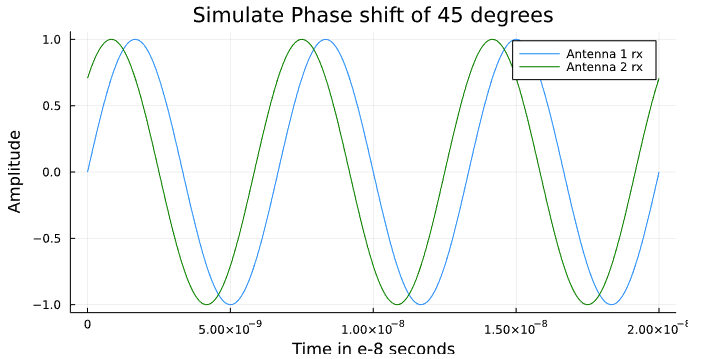
\includegraphics[width=0.8\textwidth]{Images/plots/phaseshift-sim.png}
    \caption{Result of a simulated phase shift, showing an offset of $\frac{\pi}{4}$ in Antenna 1 rx signal radians}
    \label{fig:phaseshift}
\end{figure}

An alternative method for a simulated \gls{pd} was briefly tested, and the results are displayed in table \ref{tab:shift-relative}. This method differed in that phase1 was kept constant, and a delay was added to signal $v2$ before an \gls{fft} was performed.

\begin{center}
    v2 = A$\times$ sin.($\omega_0 \times $ t. -$\phi$);
\end{center}

\begin{center}
\begin{tabular}{c|c|c|c}\centering
    \textbf{Phase1} & \textbf{Phase2} & \textbf{Phase Difference} & \textbf{$\phi $}  \\
    \hline
    350.2075549 & -349.2858886 & 3.081091629 & 5\\
    350.2075549 & -339.4949652 & 2.906325525 & 15 \\
    350.2075549 & -319.3886503 & 2.731588603 & 25\\
    350.2075549 & -271.3055298 & 2.469647073 & 40\\
    350.2075549 & -228.7212363 & 2.295114248 & 50\\
    350.2075549 & -95.19498861 & 1.859127967 & 75\\
\end{tabular}
\captionof{table}{Relative phase difference calculated from conjugate symmetry of Phase2 vs Phase1 \label{tab:shift-relative}}
\end{center}

\newpage
Remembering phase difference is calculated using:
\begin{lstlisting}
Z = p1 .* conj(p2)
phase_diff = angle(Z)
\end{lstlisting}

Phase1 \& Phase2 represent the imaginary portion of the complex \gls{iq} value at the index of the maximum magnitude in the \gls{fft}.

This validation test proved that extraction of a \gls{pd} was possible, and additionally that by virtual movement of the transmission source, induced \gls{pd} perceived at the antenna array. 

\subsection{Angle calculated vs actual angle}
With the \gls{pd} extracted, an \gls{AoA} was calculated in order to verify that the \gls{pd} represented, and aligned with the theory presented in section \ref{sec:Design/phasecalc}. The results from this section of validation tests are shown in table \ref{tab:sim-results}. For brevity in this report, table \ref{tab:sim-results} reflects a summarised version of results, and Figure \ref{fig:sim-graph} shows a plot of every calculated angle and the actual angle for more detail. 

\begin{center}
    \begin{tabular}{c|c|c}
        \textbf{Phase Difference} & \textbf{Calculated AoA} & \textbf{Actual AoA}   \\
        \hline
        1.859127967 & -63 & -75 \\ 
        2.295114248 & -43.1 & -50 \\
        2.644264734 & -32.7 & -30 \\
        2.993723168 & -14.3 & -10 \\
        3.081091629 & -9.46 & -5\\
        0 & 0 & 0\\
        -3.081091629 & 9.46 & 5\\
        -2.993723168 & 14.3 & 10\\
        -2.644264734& 32.7 & 30\\
        -2.295114248 & 43.1 & 50\\
        -1.859127967 & 63 & 75\\
    \end{tabular}
    \captionof{table}{Summarised results from simulation validation testing of Calculated AoA and Actual AoA \label{tab:sim-results}}
\end{center}

*Note that a $-ve$ degree angle is evidence of transmission source on the \emph{left} hand side of the euclidean coordinate system, as represented in Figure \ref{fig:phase-change}. 

\begin{figure}[h]
    \centering
    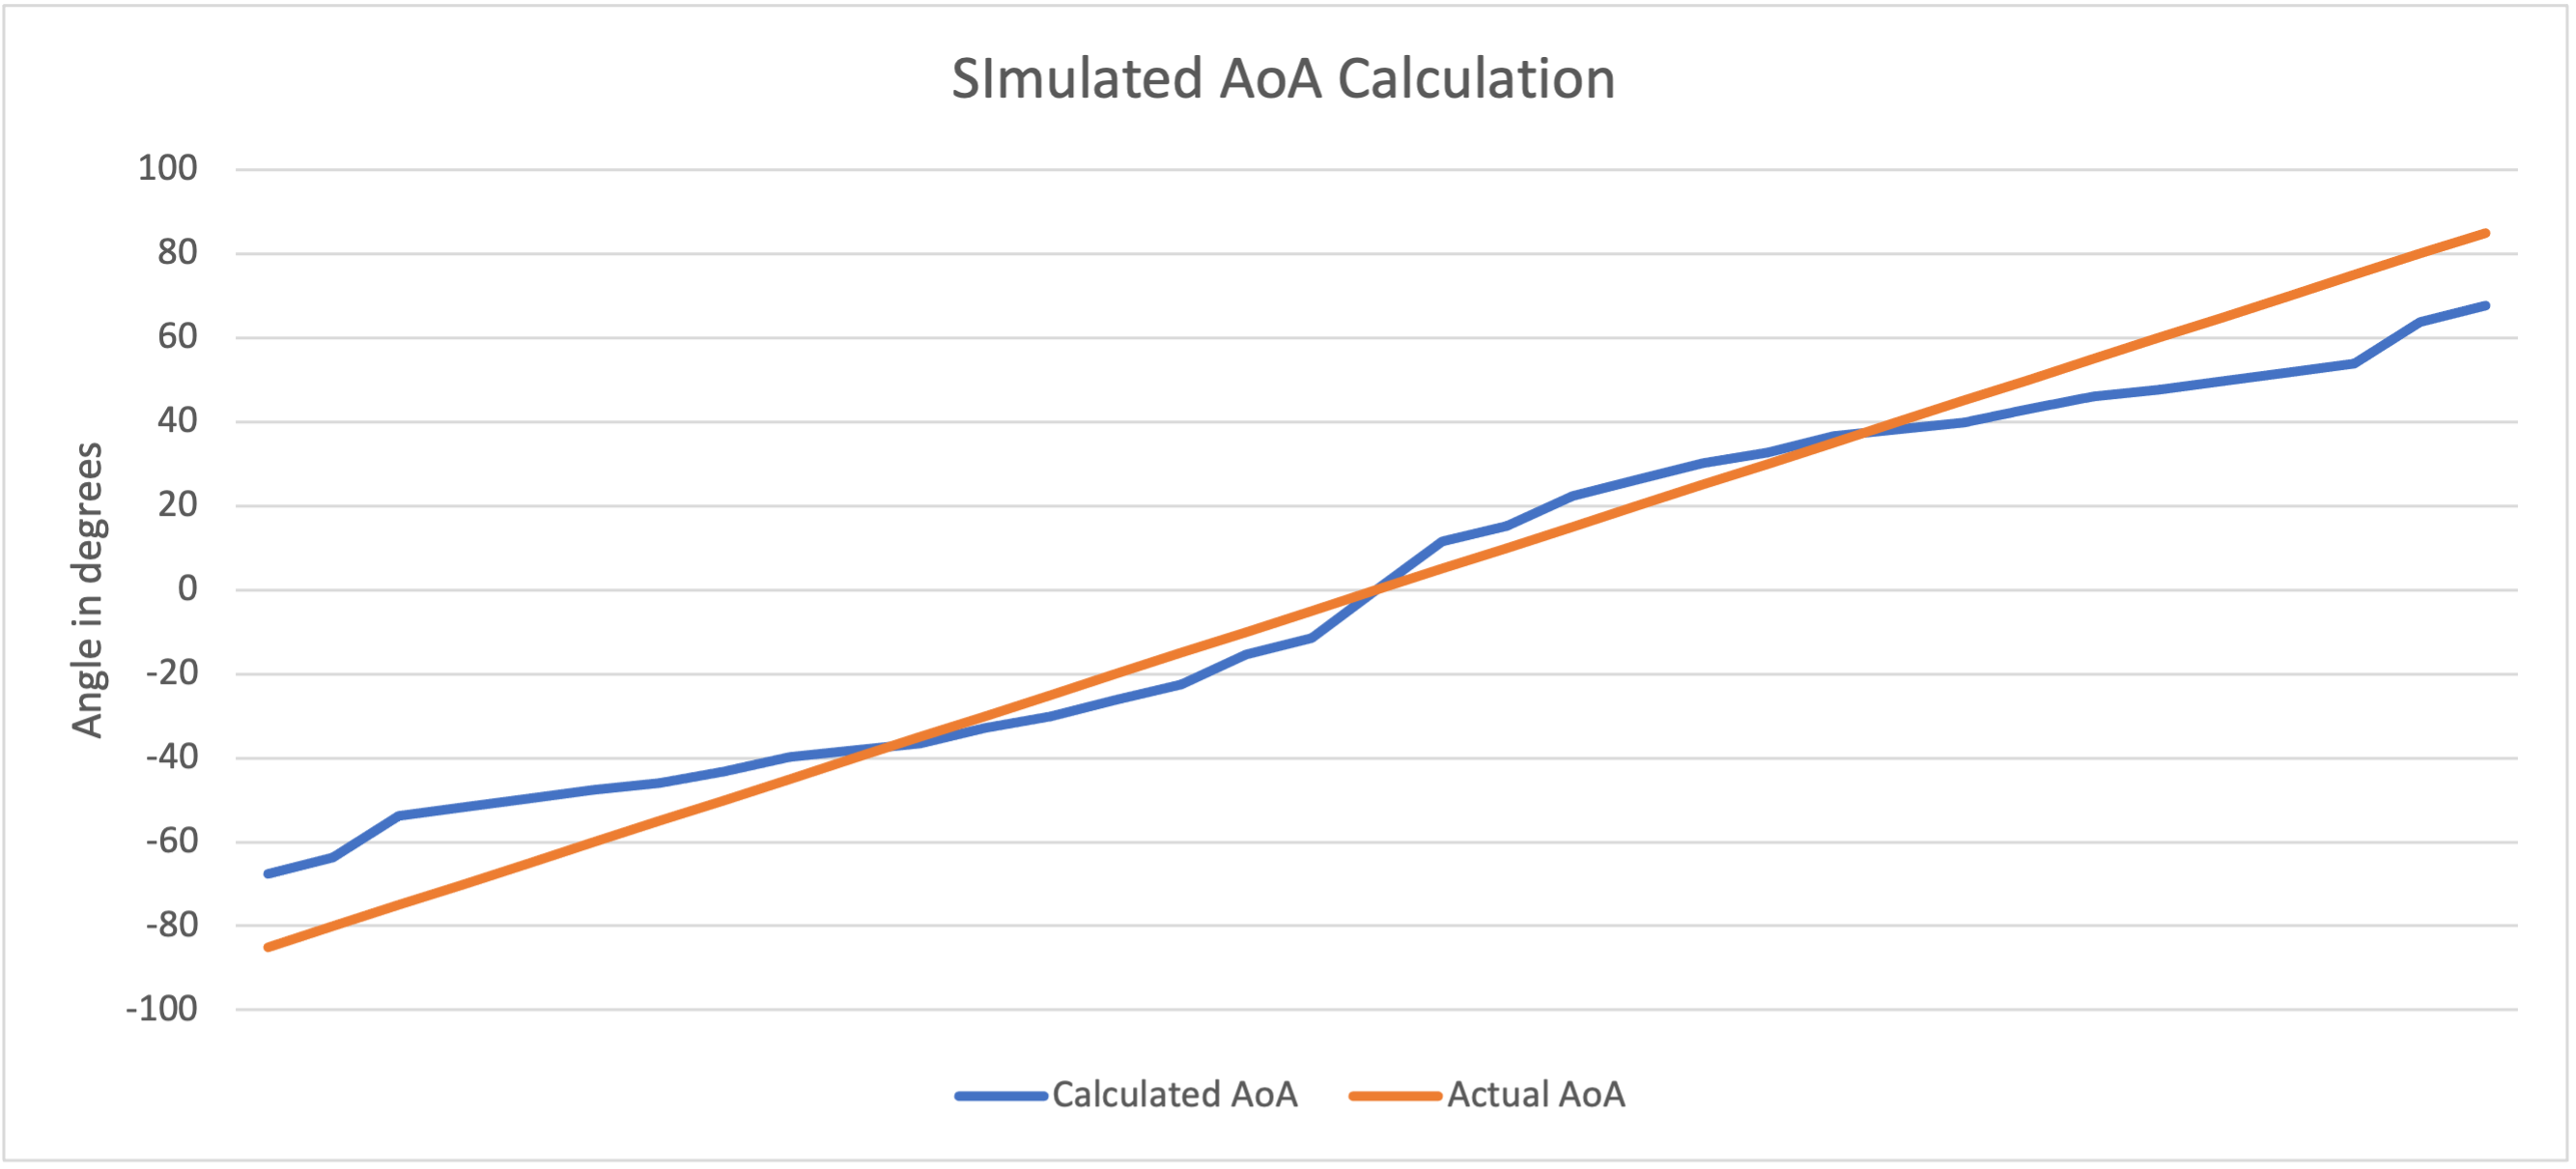
\includegraphics[width=0.9\textwidth]{Images/plots/simulatedaoa.png}
    \caption{Simulation AoA calculation and Actual AoA, showing the difference between the results}
    \label{fig:sim-graph}
\end{figure}

\subsection{Mean Squared Error}
During the course of this project, it has become apparent that the more data that is collected, the less error should occur. While not the case for this simulation as the precision of the data types does not change, nor will the phase values calculated as there is no noise within the data, this is certainly the case for the real-world prototype. As an introduction to the \gls{mse}, and for use in comparison to the prototype built, the \gls{mse} is calculated for the simulated data results collected above.

\begin{equation}
    MSE = \frac{1}{N} \sum_1^N{(Y_i - \hat{Y_i})}
\end{equation}

\textbf{MSE For simulated data} = 120.173

This will be relative in section \ref{sec:results-stats}, when comparing to the normal distribution of the data.

\section{Prototype Project Results}
%---------------------------------
% Time aligned signals
%---------------------------------
This section details the majority of data collection in terms of results for this project, and the associated analysis of said results. The validation tests here are aimed at proving the successful implementation of the project's goal, which to reiterate was to \emph{prove that through movement in a transmission source, the resulting phase shift can be extracted for two \gls{rx} antenna, using a \gls{sdr}}.

\subsection{Time-aligned \& synchronised signal}
The first validation that was needed to be confirmed was the time alignment of signals. This was an oversight of this project, as it itself was not thoroughly investigated, however, the time synchronisation of the LimeSDR, and GNU Radio scheduler allowed for usable, if not controllable sampling. Additionally, as seen in Figure \ref{fig:lime-clipping}, there was unknown behaviour of the \gls{sdr} board that should be further investigated for its effect in this regard. At this stage, to view if sampled \gls{rf} signals are time-aligned, \gls{fm} modulated signals at 89MHz are sampled using the methodology discussed in Chapter \ref{ch:meth} and viewed in the time domain in Figure~\ref{fig:time-align}.

\begin{figure}[h]
    \centering
    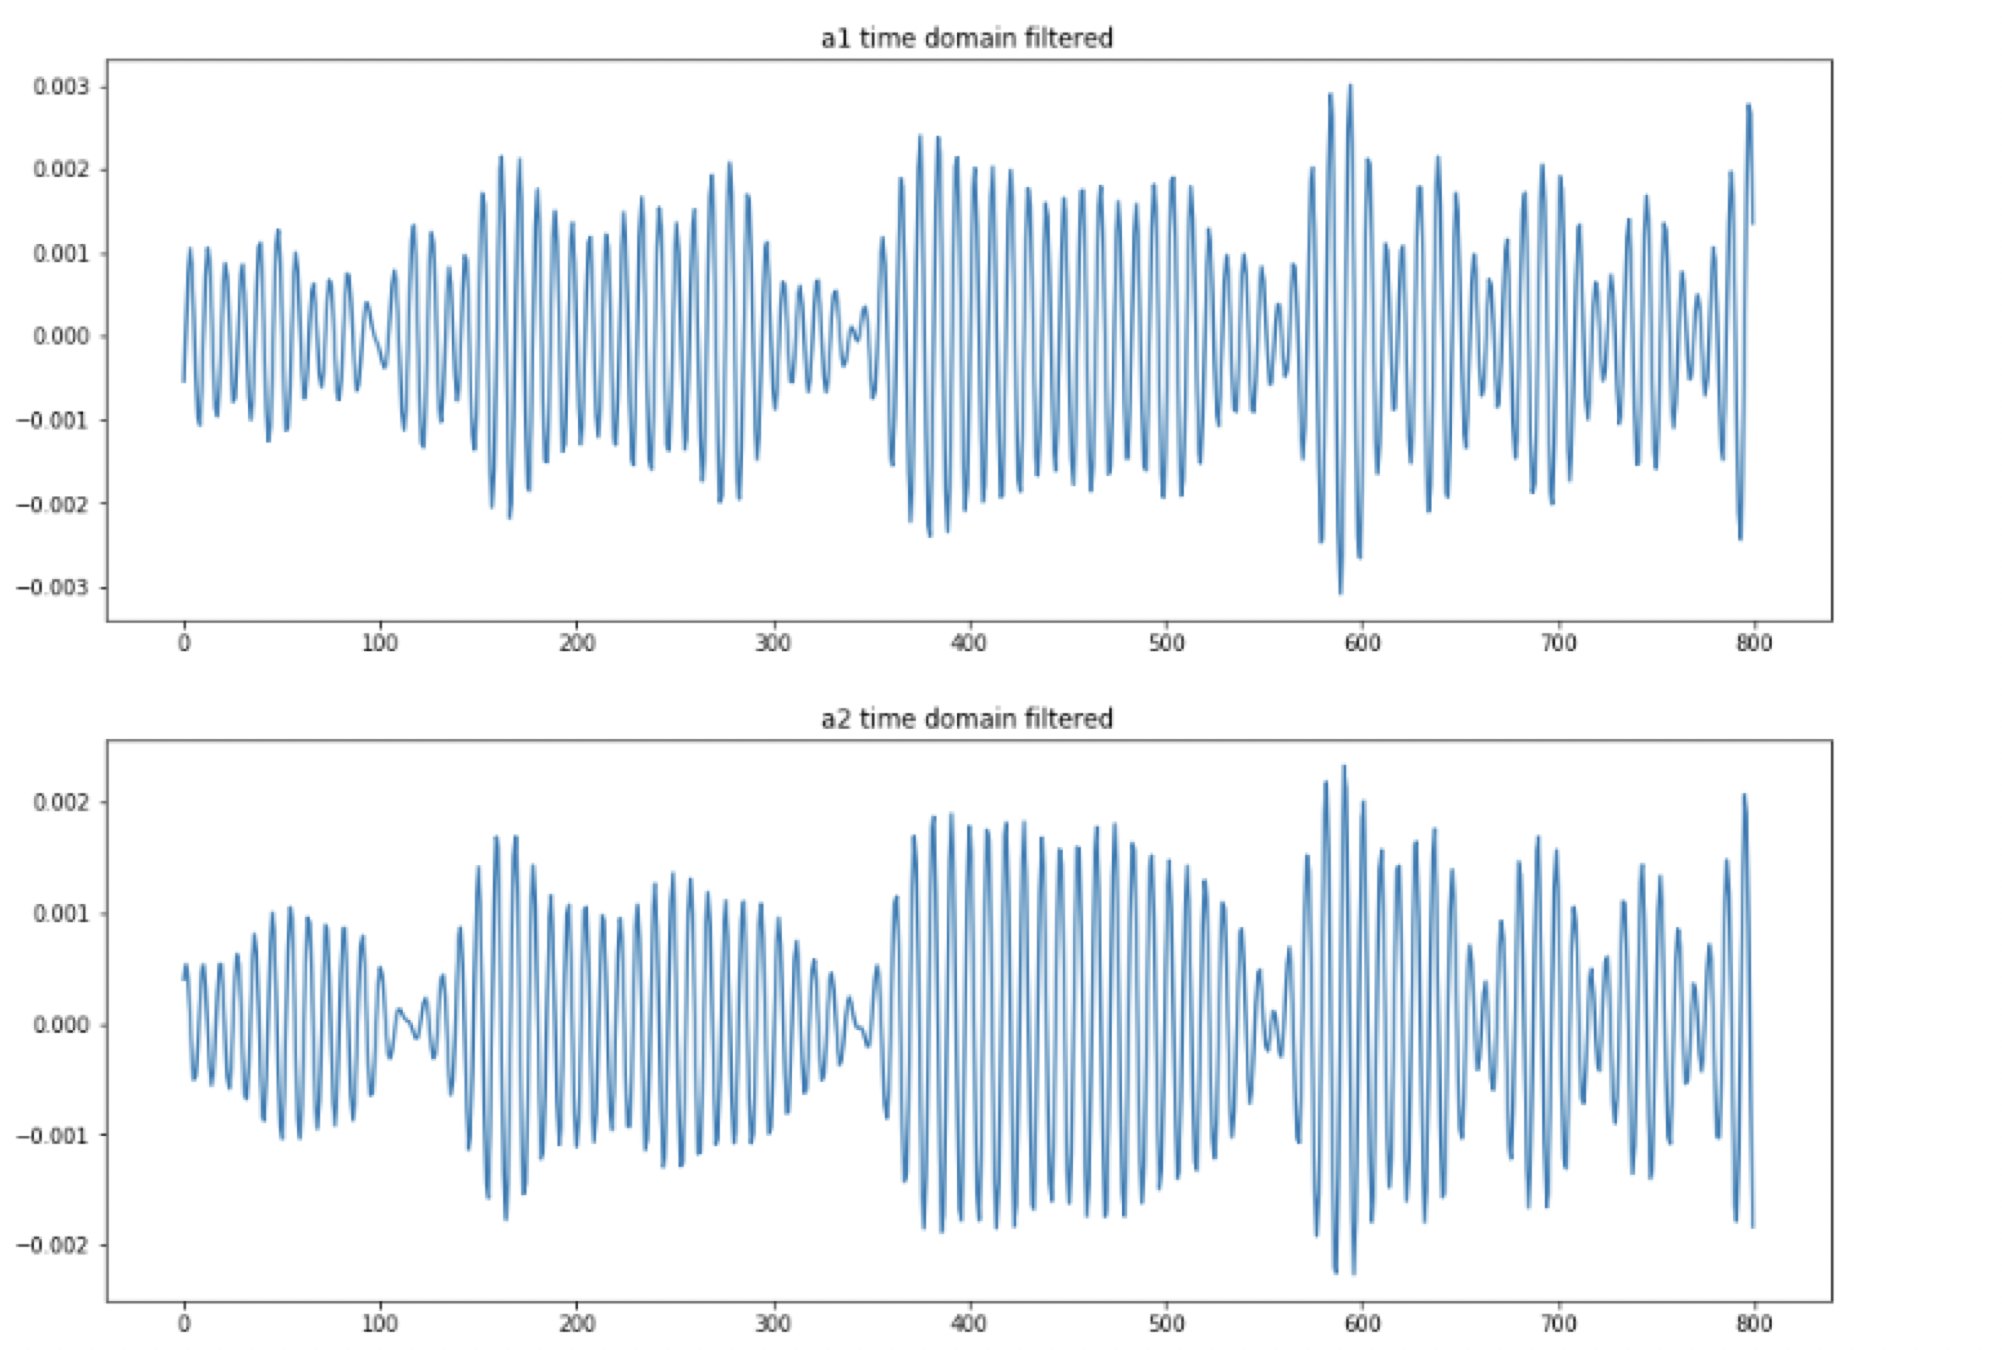
\includegraphics[width=0.8\textwidth]{Images/plots/time relation.png}
    \caption{Both A1 and A2 received signals correlation in the time domain shown}
    \label{fig:time-align}
\end{figure}

The signals appear to have a correlation, and thus the project proceeded with testing of phase calculations, which would further confirm if the data is time-aligned.

By viewing the real portion of the sampled data side-by-side in Figure \ref{fig:inverse}, there is clear evidence of an inverse relation, with changes occurring at the same sample. This suggested a 180 phase offset in the received data, but proves that the data is sampled synchronously.  

\begin{figure}[h!]
    \vspace{0.5cm}
    \centering
    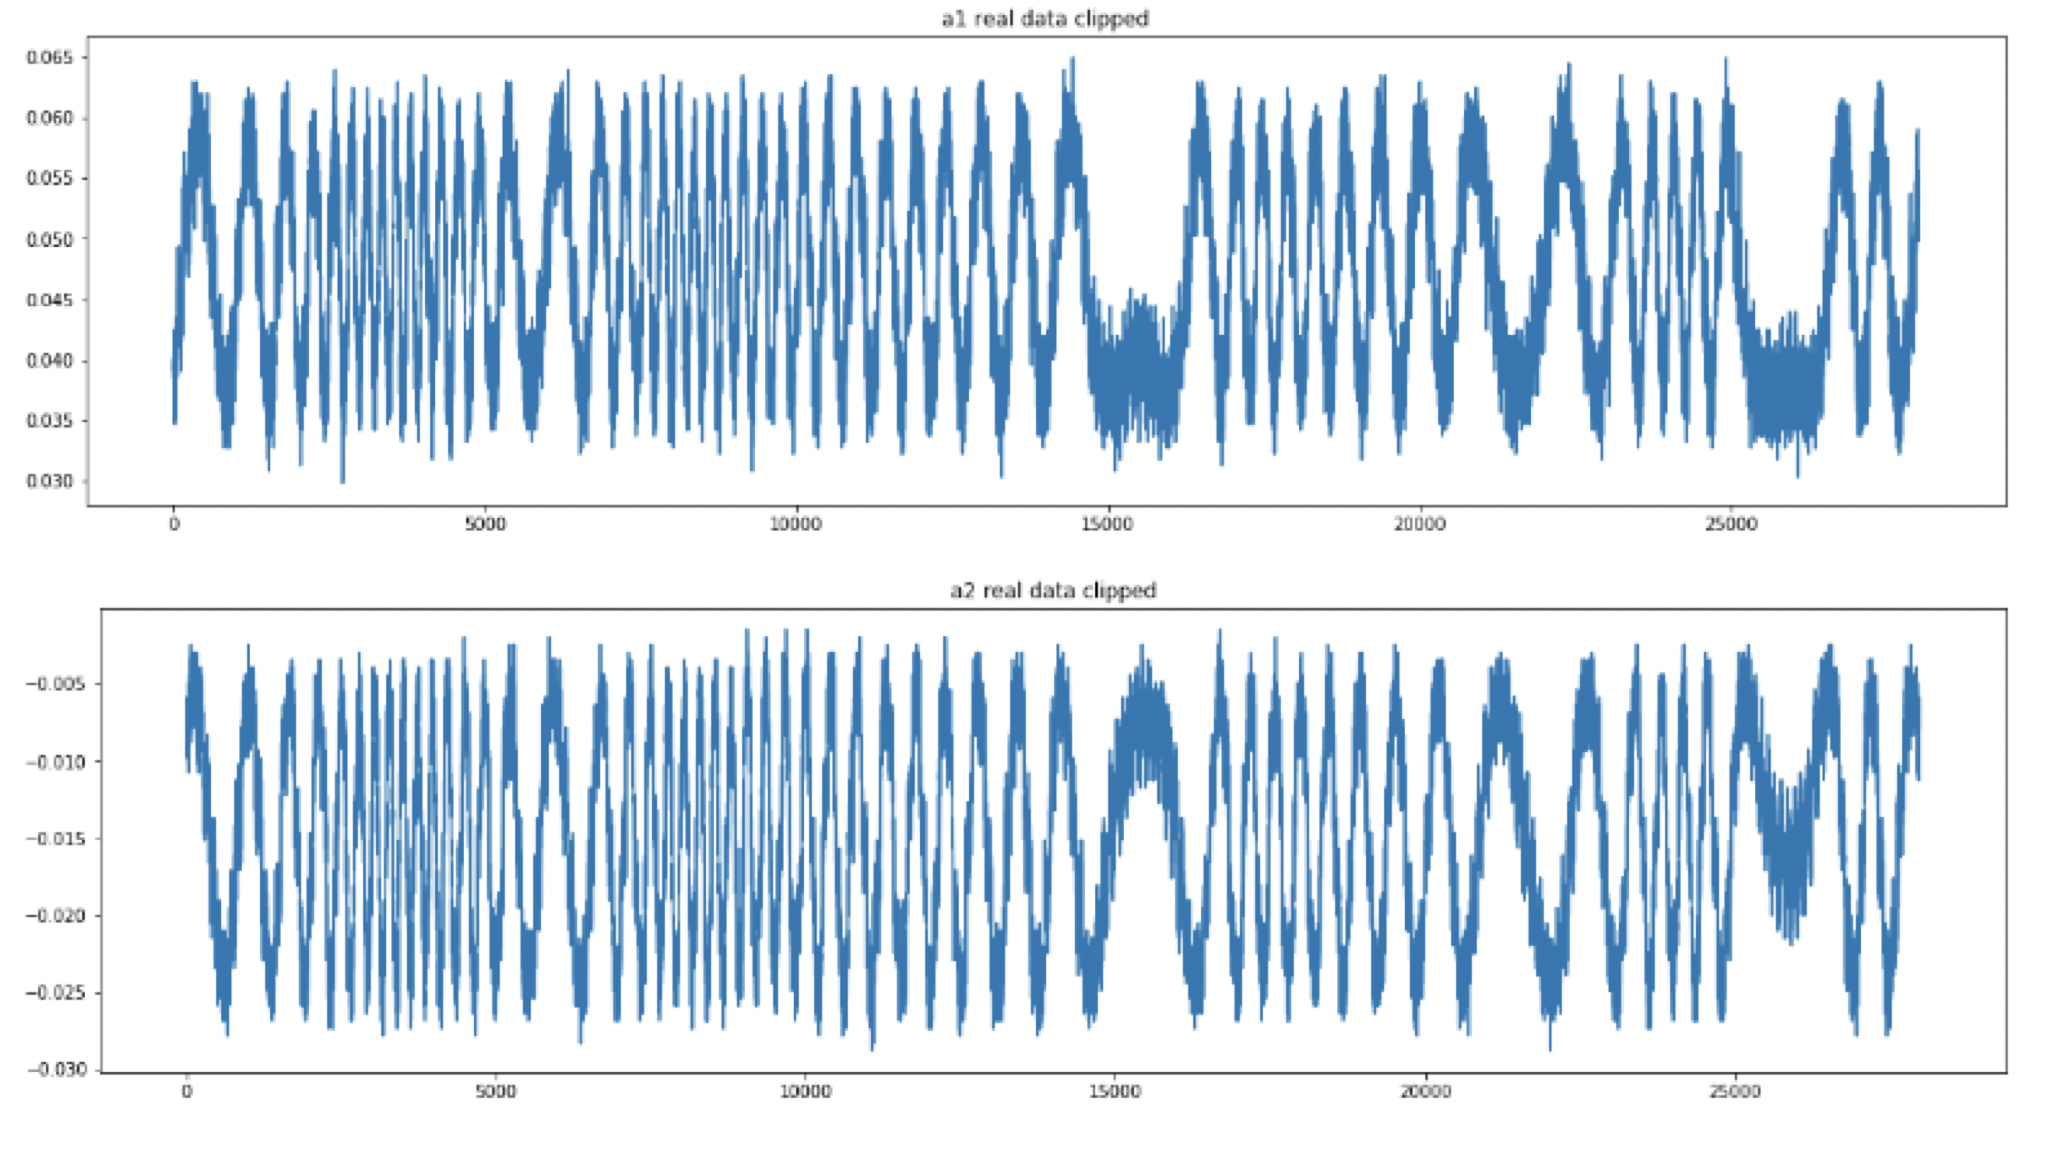
\includegraphics[width=0.8\textwidth]{Images/plots/inverserelation.png}
    \caption{Inverse and relationship between A1 and A2 signals, real portion.}
    \label{fig:inverse}
\end{figure}

Viewing the constellation of the \gls{iq} data from each \gls{rx} antenna shows additional information regarding the signal. For data received in this project, plotting I vs Q as shown in Figure~\ref{fig:IQconst} shows the polar coordinates of the received signals. In this plot, the majority of samples sit on or near a multiple of the unit circle. The phase noise can be seen by multiple circles or data occurring with each circle having an increased radius.

\begin{figure}[h!]\centering
    \subfloat[A1 constellation]{\label{a}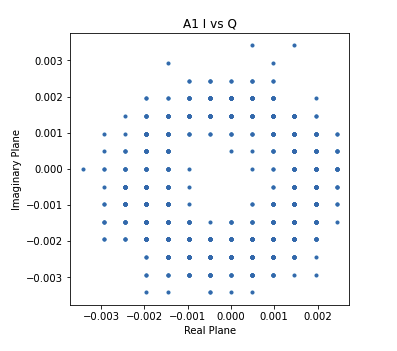
\includegraphics[width=.45\linewidth]{Images/plots/a1-IQ.png}}
    \subfloat[A2 constellation]{\label{b}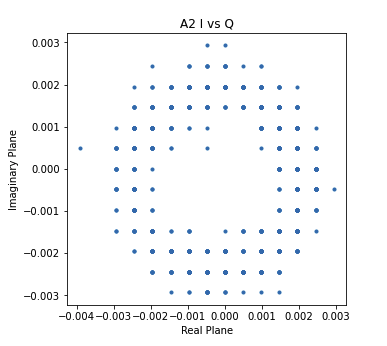
\includegraphics[width=.45\linewidth]{Images/plots/a2-IQ.png}}\hfill 
    \caption{I vs Q Constellation Plots from each Rx antenna.}
    \label{fig:IQconst}
\end{figure}
%---------------------------------
% DC Offset 
%--------------------------------
\subsection{DC Offset removal}
As per listing \ref{lst-dc}, removal of the DC offset caused by the \gls{lo} frequency was performed in \textsc{Python}. The \gls{lo} spike can be seen at centre frequency 150MHz, shown in Figure \ref{fig:dc-spike}, and the same sampled data with the \gls{lo} spike removed in Figure \ref{fig:dc-spike-remove}. This proved highly successful. 

\begin{figure}[!h]
    \centering
    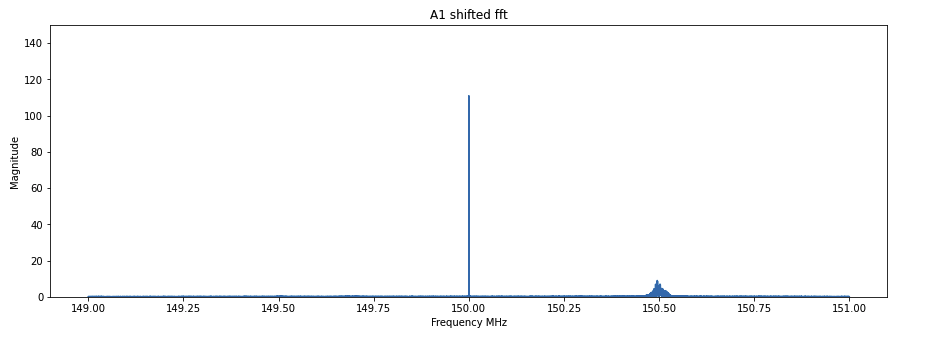
\includegraphics[width=0.8\textwidth]{Images/plots/dcspike.png}
    \caption{LO DC Frequency component seen at centre frequency as a result of mixing}
    \label{fig:dc-spike}
\end{figure}

\begin{figure}[!h]
    \centering
    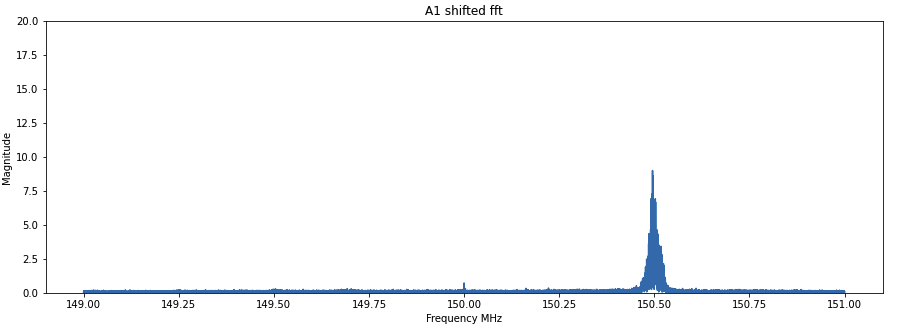
\includegraphics[width=0.8\textwidth]{Images/plots/dcspike-remove.png}
    \caption{DC Spike from LO, as shown in \ref{fig:dc-spike}, removed through \textsc{Python} code}
    \label{fig:dc-spike-remove}
\end{figure}


%---------------------------------
% Phase Calculation Angle
%---------------------------------
\subsection{Change in Phase}
Following the methodology layout in Chapter \ref{ch:meth} for experimental collection, and adhered to in section \ref{sec:results-sim}, the phase extracted without averaging is presented in the tables \ref{tab:phase-results} and \ref{tab:phase-results1}. The angle denoted by  $\phi$ represents the actual angle of arrival from the testing experiments. This table represents the entire range of angles measured but does not include each angle, rather this is shown in Figure \ref{fig:phase-angles}.

Note, that this is a single-phase extracted for each defined angle, and not averaged as of yet. Data is captured one 0.1second, and the phase extracted from the complex number at the index in the array of the where the maximum value of the magnitude of the \gls{fft} occurs.

\centerline{\emph{where: Phase1= angle(p1) and p1 is complex}}
\vspace{0.5cm}

\begin{minipage}[!h]{.48\linewidth}\centering
\begin{center}
    \begin{tabular}{c|c|c|c|}
        \textbf{Phase1} & \textbf{Phase2} & \textbf{\gls{pd}} & \textbf{$\phi $}   \\
        \hline
        -0.3109310 & 0.4789530947 & 0.168022 & 0 \\
        0.0102383 & 0.0102383 & 0.1687452 & -5 \\
        -0.129312 & -0.201397 & -0.33071 & -10 \\
        -1.239082 & 1.125299 & -0.113783 & -15 \\
        -3.123897 & 1.687016 & -1.4368809 & -25 \\
        -2.498529 & 1.325405 &  -1.17312396& -50 \\
        -3.231939 & 1.046477 & -2.18546226 & -65 \\
        -2.390812 & 0.0713802 & -2.31943268 & -80 \\
    \end{tabular}
    \captionof{table}{Non-Averaged Phase at each antenna for negative angless \label{tab:phase-results}}
\end{center}
\end{minipage}%
\hspace{0.2cm}
\begin{minipage}[!h]{.48\linewidth}\centering
\begin{center}
    \begin{tabular}{c|c|c|c|}
        \textbf{Phase1} & \textbf{Phase2} & \textbf{\gls{pd}} & \textbf{$\phi $}   \\
        \hline
        -0.0128462 & -0.0455013 & -0.058347 & 0 \\
        0.19873465 &  0.0206113 & 0.219346 & 5 \\
        0.6982491 & 0.1712281 & 0.8694773 & 10 \\
        0.6984230 & 0.2146852 & 0.9131083 & 15 \\
        1.2309852 & 0.5259291 & 1.7569143 & 25 \\
        1.7240983 &  0.36964 & 2.0937391 & 50 \\
        0.938578 & 0.2460543 & 1.184632 & 65 \\
        2.1498637 & 0.4960692 & 2.645933 & 80 \\
    \end{tabular}
    \captionof{table}{Non-Averaged Phase at each antenna for positive angles \label{tab:phase-results1}}
\end{center}
\end{minipage}

\begin{figure}[h]
    \centering
    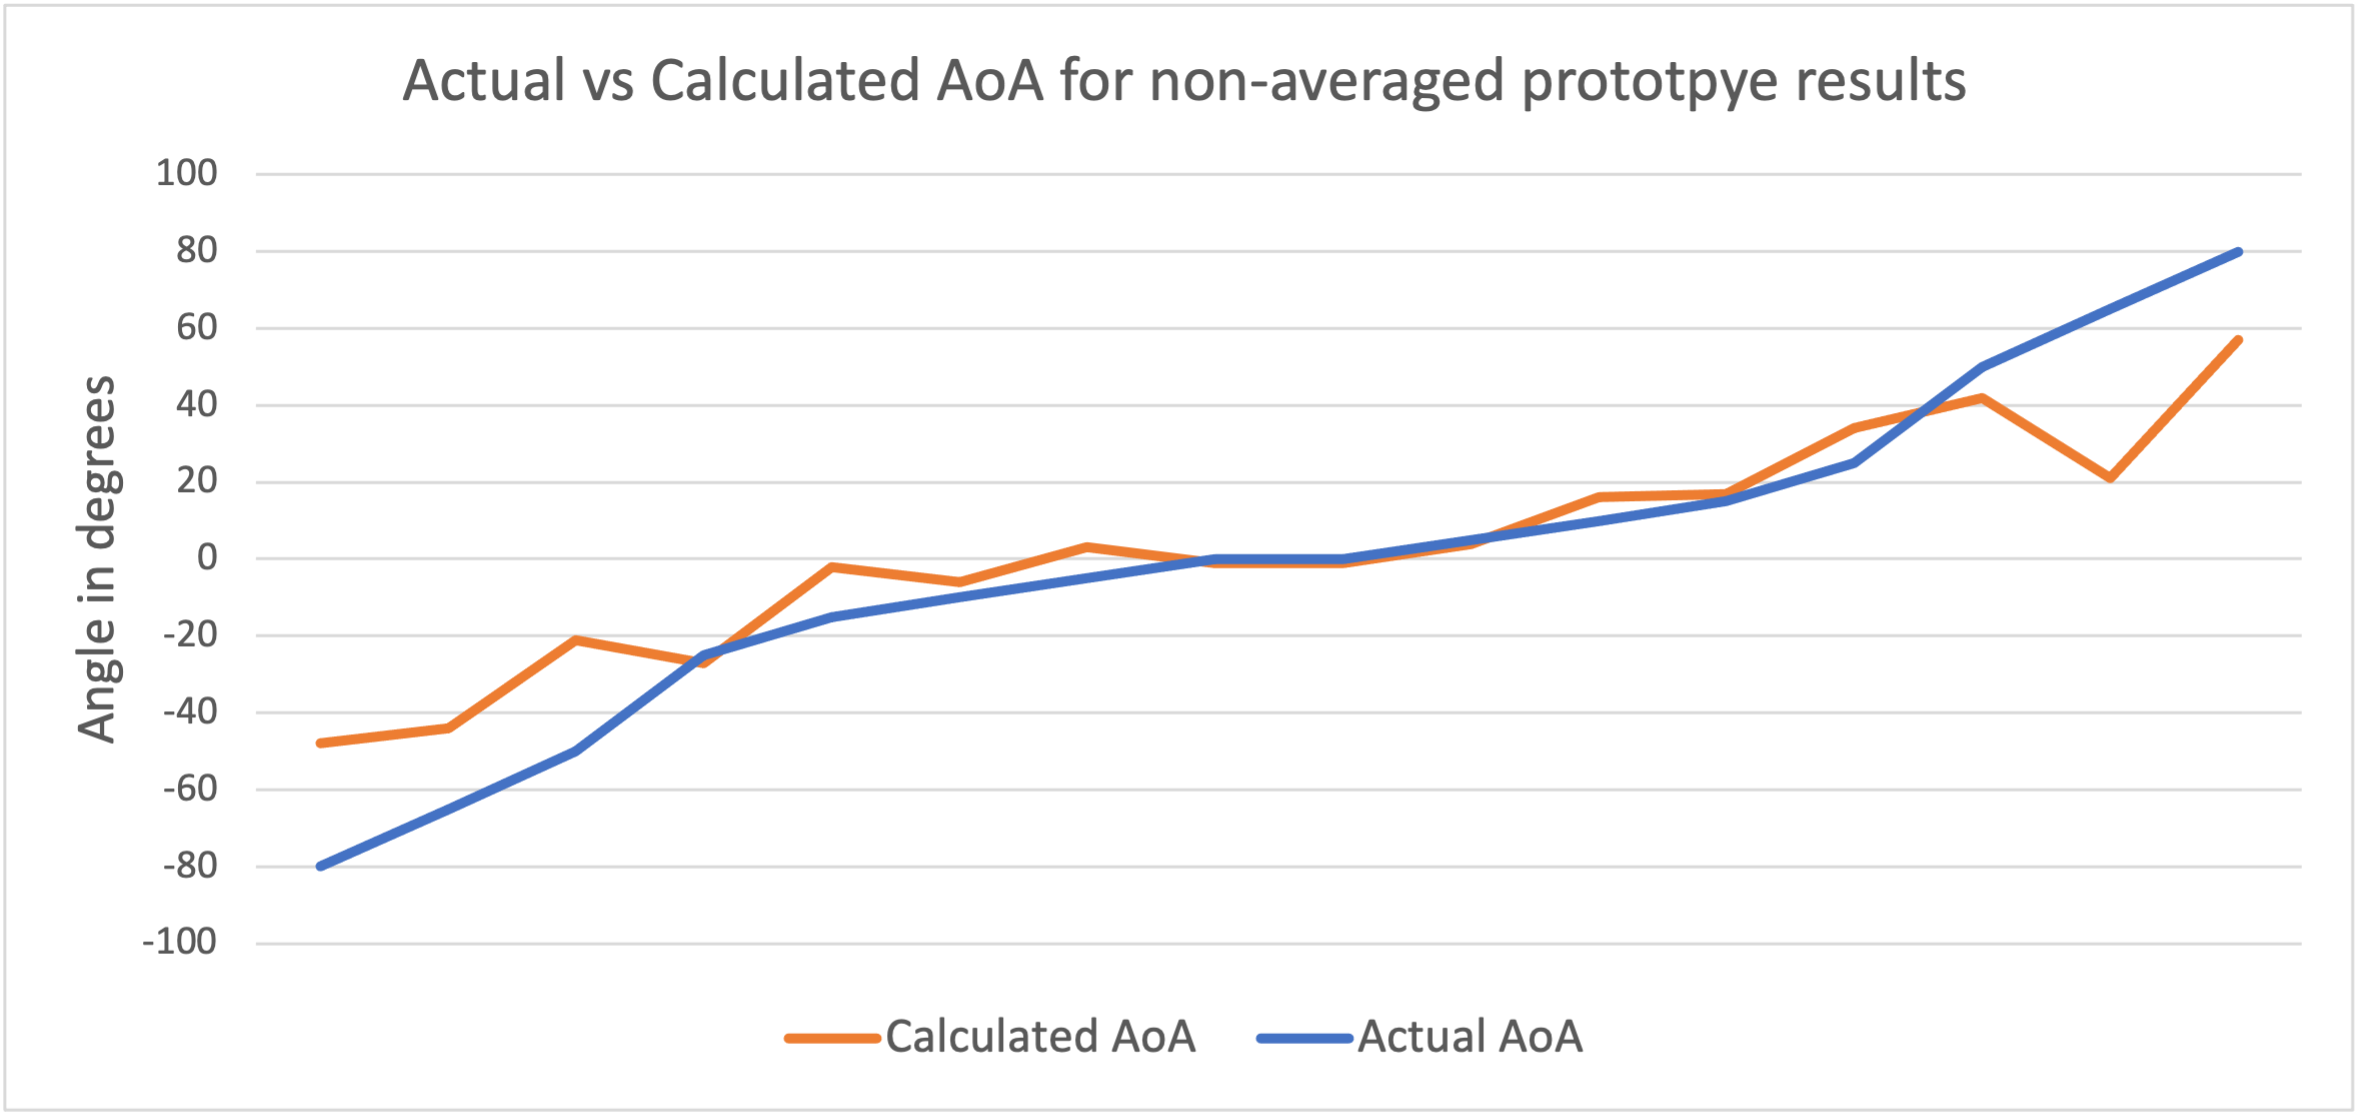
\includegraphics[width=0.9\textwidth]{Images/plots/AoA-prototpye-nonaveraged.png}
    \caption{Comparison of the calculated AoA vs the actual AoA, with no averaging}
    \label{fig:phase-angles}
\end{figure}

\subsection{Averaged Phased results}
In briefly providing tables \ref{tab:average-p} and \ref{tab:average-p1} here, the results of averaging \textbf{20 extracted phasors without moving the transmission source} is shown. This is to be further analysed in section \ref{sec:results-stats}, noting that the averaging performed in this manner is of the complex phasor at the maximum of the magnitude \gls{fft} signal, before any phase extraction. After the averaging, the \gls{pd} is then calculated. This allows the phase induced by noise and reflections to be beaten, resulting in a more accurate phasor to use in figure \ref{fig:average-phase} 

\begin{minipage}[h!]{.45\linewidth}\centering
\begin{center}
    \begin{tabular}{c|c}
        \textbf{Angle $\phi$} & Averaged Phasor \gls{pd} \\
        \hline
        0 & 0.168022\\
        -5 & 0.056731 \\
        -10 & -0.438711 \\
        -15 & 0.65412\\
        -25 & -0.97339\\
        -50 & -1.0759028\\
        -65 & -1.8479724\\
        -80 & -2.336123 \\
    \end{tabular}
    \captionof{table}{Averaged Phasor PD, negative angles (degrees) \label{tab:average-p}}
\end{center}
\end{minipage}%
\hspace{0.5cm}
\begin{minipage}[h!]{.45\linewidth}\centering
\begin{center}
    \begin{tabular}{c|c}
    \textbf{Angle $\phi$} & Averaged Phasor \gls{pd} \\
        \hline
        0 & 0.168022\\
        5 & 0.65398\\
        10 & 0.71286\\
        15 & 0.98443\\
        25 & 0.438711\\
        50 & 1.77259\\
        65 & 2.1418056\\
        80 & 2.195384\\
    \end{tabular}
    \captionof{table}{Averaged Phasor PD, positive angles (degrees) \label{tab:average-p1}}
\end{center}
\end{minipage}

In tables \ref{tab:average-p} and \ref{tab:average-p1}, the \textbf{Angle $\phi$} is the actual \gls{AoA} defined during validation, and not the calculated \gls{AoA}.

\subsection{Angle calculated vs actual angle}
Similar to the simulation validation, Figure \ref{fig:average-phase} provides a graph of the calculated \gls{AoA} plotted with the Actual \gls{AoA} for comparison. The calculated \gls{AoA} uses the averaged \gls{pd} from tables \ref{tab:average-p} and \ref{tab:average-p1}. While this is not accurate, especially when compared to the simulation in Figure \ref{fig:sim-graph}, it does however show that the \gls{pd} does follow the transmission source, and thus proves the workings of this system. Further investigation into the averaging, correlation and length of samples would be needed for a more accurate \gls{AoA} to be produced. 

\begin{figure}[h]
    \centering
    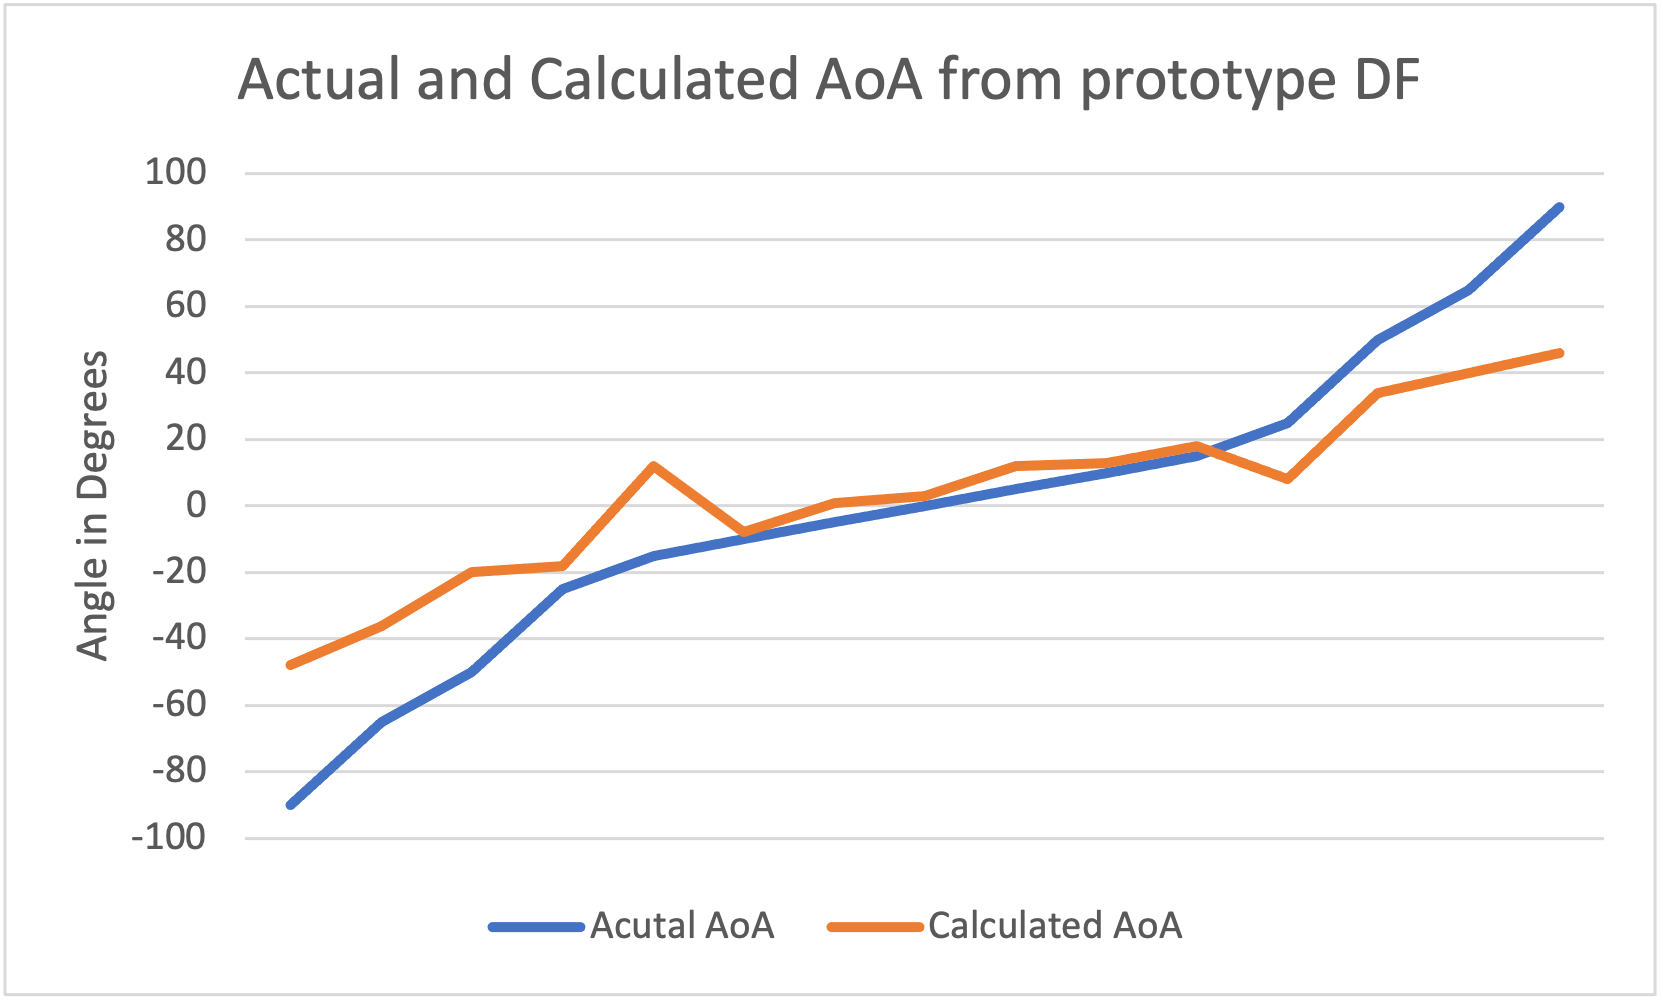
\includegraphics[width=13cm,height=7.2cm]{Images/plots/AoA-prototype.png}
    \caption{Calculated AoA from the system prototype compared to the actual AoA}
    \label{fig:average-phase}
\end{figure}

%---------------------------------
% Statistically Analysis
%---------------------------------
\section{Statistical Analysis \label{sec:results-stats}}
In order to further analyse the samples received from the \gls{sdr}, a validation test was performed to view the statistical distribution of the extracted \gls{pd}, with no change in the transmission sources location. With noise and reflections affecting the phase measurement, the extracted phase is not constant. This should however fit into a normal distribution if the noise is random, and not introduced by the \gls{sdr}.

\subsection{Averaged Data}
The mean, standard deviation and \gls{mse} calculated for this validation are all calculated from data which is produced from a static transmission source, one thousand (1 000) iterations and the \gls{pd} for each iteration calculated. 

\subsubsection{Arithmetic Mean}
The data was collected over one thousand (1 000) iterations, with a constant position of the antenna array and the transmission source, all within a lab. The transmission source was first placed perpendicular to the antenna array which should result in zero phase shift between the two antennas and then placed at positive twenty-five (25) degrees for a further one thousand (1 000) iterations.

\begin{center}
    \begin{tabular}{c|c|c}
        \textbf{Actual Angle $\phi$} & Previous Phasor \gls{pd} & Calculated \gls{AoA}\\
        \hline
        0 & 0.168022 & 3.0636\\
        \vspace{0.5cm}
        25 & 0.438711 & 8\\
        \textbf{Angle $\phi$} & Averaged Phasor \gls{pd} over 1000 iterations & Calculated \gls{AoA}\\
        \hline
        0 & -0.04760950286 & -0.86\\ 
        25 & 1.1875606802 & 22.19 \\
    \end{tabular}
    \captionof{table}{Averaging the Phasor over 1 000 iterations brings the calculated \gls{AoA} closer to the actual \gls{AoA} (reducing error) \label{tab:proof-of-averaging}}
\end{center}

Table \ref{tab:proof-of-averaging} clearly shows the improvement made by averaging over one thousand iterations. While this is not practically possible in a real-world application, it has validated the system further and shown the benefit of averaging of the phasor before phase \gls{AoA}.

Additionally, as the calculation of the \gls{AoA} is a non-linear function of phase, the improved results are significant due to the amount of noise in the received signal. 

\subsubsection{Standard Deviation}

The standard deviation of phase from one thousand (1 000) iterations is:
\begin{equation*}
    STD = 0.405450582
\end{equation*}
With the mean already calculated as \textbf{-0.04760950286}, the conlusion is that the majoirty of the data will fall within \textbf{mean} $\pm$ \textbf{STD}

\begin{center}
    \begin{tabular}{c|c|c|c}
        & -STD & mean & + STD  \\
        \hline
        \gls{pd} & -0.4530600849 & -0.04760950286 & 0.3578410791 \\
        \gls{AoA} & -8.2 & -0.8 & 6.5\\
    \end{tabular}
    \captionof{table}{Normal distribution of data as a variation of the STD with regards to the mean for phases averaged over 1 000 iterations. \label{tab:my_label}}
\end{center}

\subsubsection{Histogram}
This can be represented in the histogram in Figure \ref{fig:hist}, showing the extracted phase falling into a normal distribution. With the mean and mode at 0 degrees, the centre of the histogram falls nicely into the normal distribution of the data. The data is varied around the mean by the standard deviation caused by errors in the phase extraction. The minimum phase is -1.92, and the maximum phase is 1.89. However, this again shows that the mean of the phases over one thousand (1 000) iterations is -0.86, shown in table \ref{tab:proof-of-averaging}, with the true mean of the data being 0.  

There is however some phenomena causing a slight increase in data frequency at the tails of the histogram, making the data not fit completely to the normal distribution. Further investigation would be needed to determine the source of this error. 

\begin{figure}[h]
    \centering
    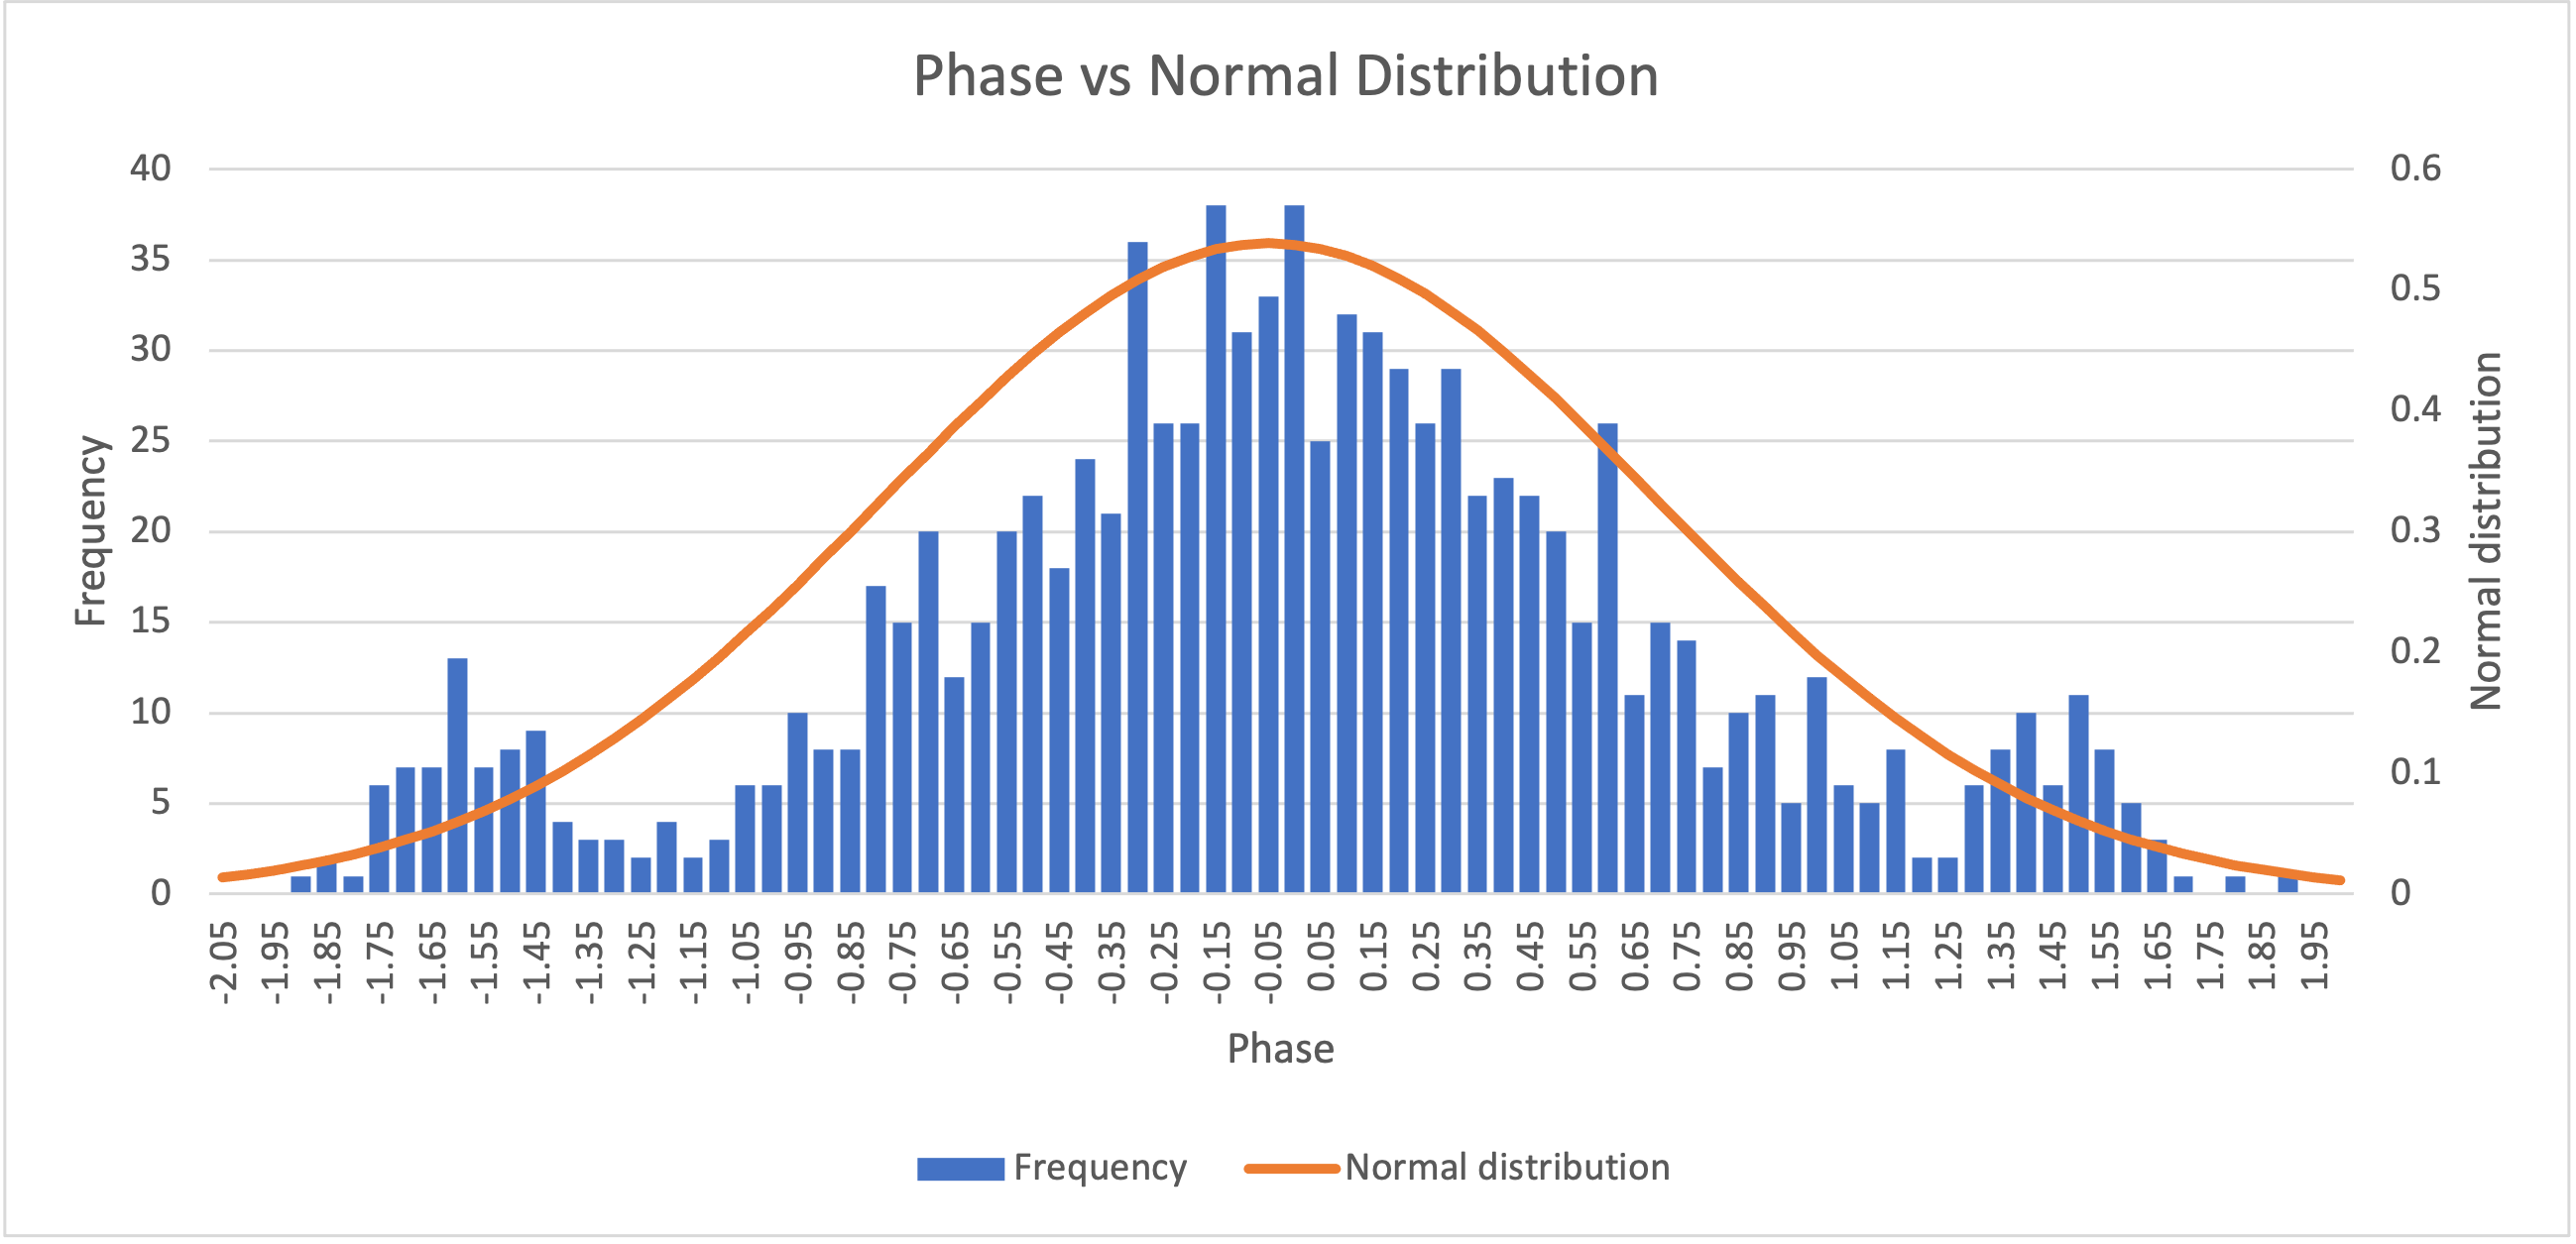
\includegraphics[width=0.8\textwidth]{Images/plots/phaseandnormal.png}
    \caption{Normal distribution fitted to a histogram for 1 000 iterations of phase extraction from static transmission source}
    \label{fig:hist}
\end{figure}


\subsection{Sample Length}
The final validation test performed was varying the sample length of the captured \gls{fft} data, to verify the theory that performing an \gls{fft}, and extracting the phase on a sample of one (1) second is more beneficial than taking one hundred (100) 0.01 second data captures and performing an \gls{fft} on those. This would benefit the \gls{SNR}. 

\begin{table}[h]
    \centering
    \begin{tabular}{c|c|c}
         & \textbf{0.01 second } &\textbf{1 second} \\
         \hline
        mean & -0.04760950286 & -0.0648721096\\
        STD & 0.7405450582 & 0.63482167\\
        MSE & 0.550125241 & NA \\
    \end{tabular}
    \caption{Comparison of statistical parameters for 0.01 seconds data capture vs 1 second data}
    \label{tab:varied-length}
\end{table}

From table \ref{tab:varied-length} the conclusion drawn is that there is no significant benefit in varying the sample length and averaging shorter sampled lengths. This is due to the relatively high \gls{SNR} in the testing environment (where reflected signals formed the majority of noise) as the signal generator had a high output dBm. 
%---------------------------------
% Sensitivity
%---------------------------------
\section{Sensitivity analysis}
The sensitivity of the \gls{AoA} calculation can be shown by plotting the error between the actual \gls{AoA} and the calculated \gls{AoA}. 

\begin{figure}[htp]
\centering\begin{subfigure}[b]{0.5\linewidth} 
\centering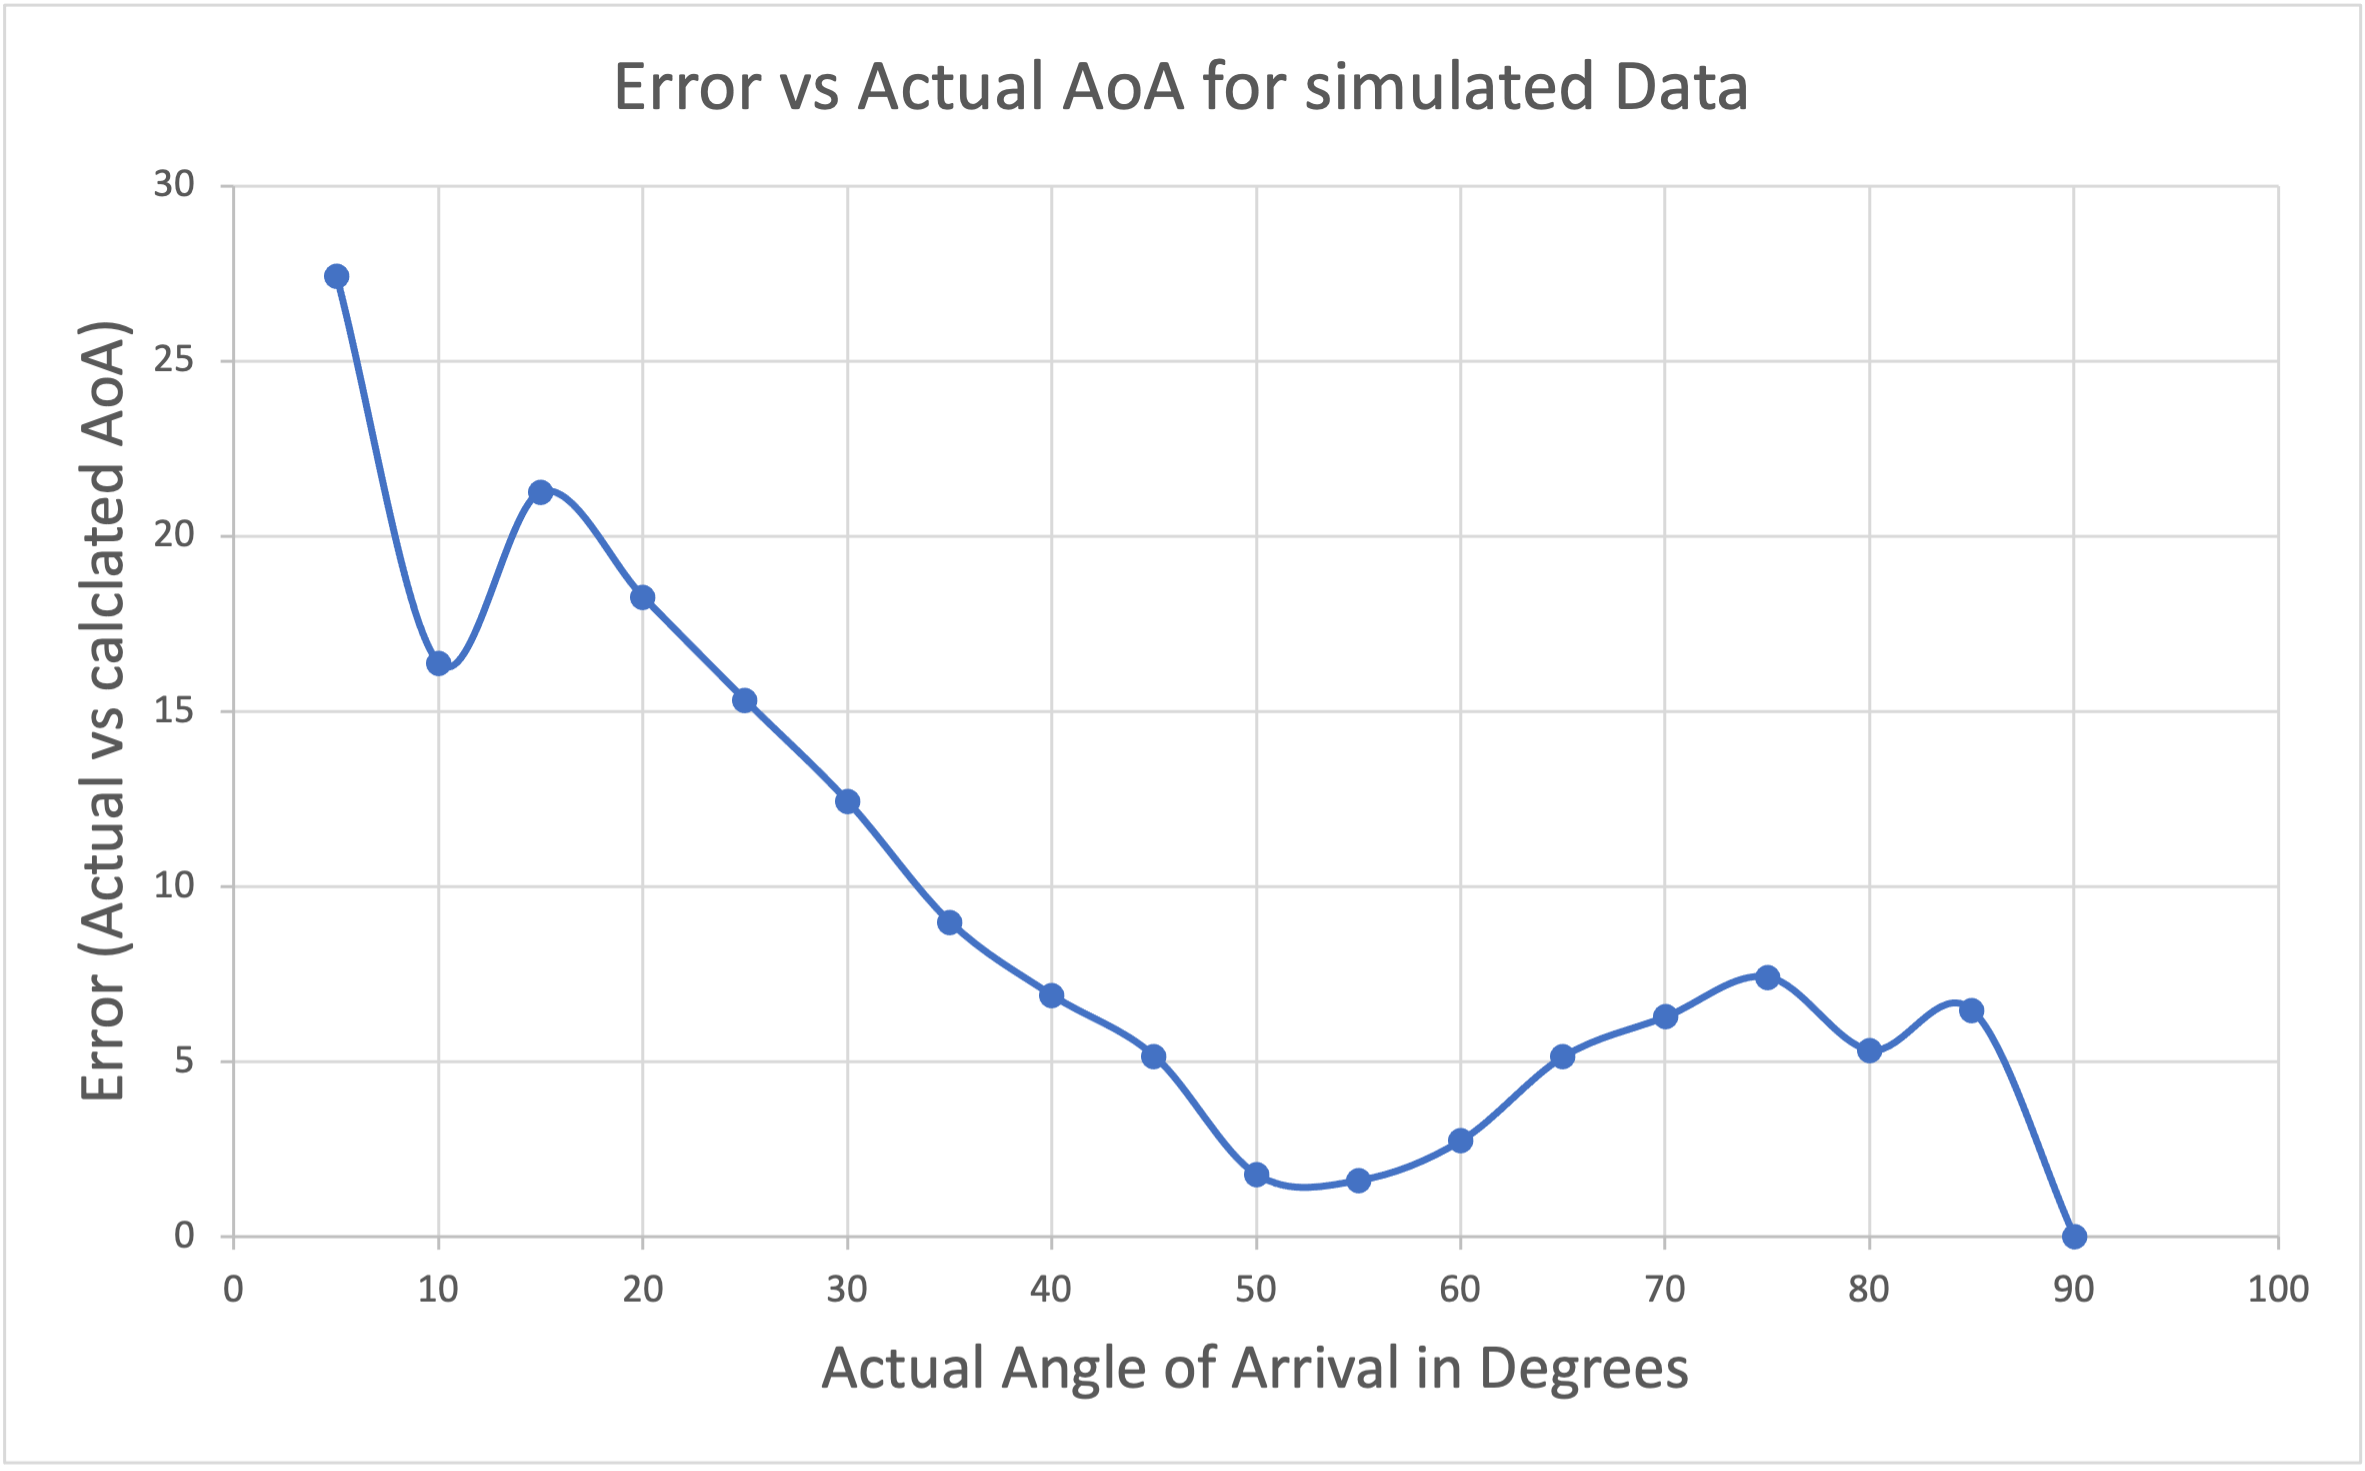
\includegraphics[width=0.88\textwidth]{Images/plots/sensitivity-sim.png} 
\caption{\label{fig:sim-error}Error sensitivity of simulation } 
\end{subfigure}\hfill
\begin{subfigure}[b]{0.5\linewidth} 
\centering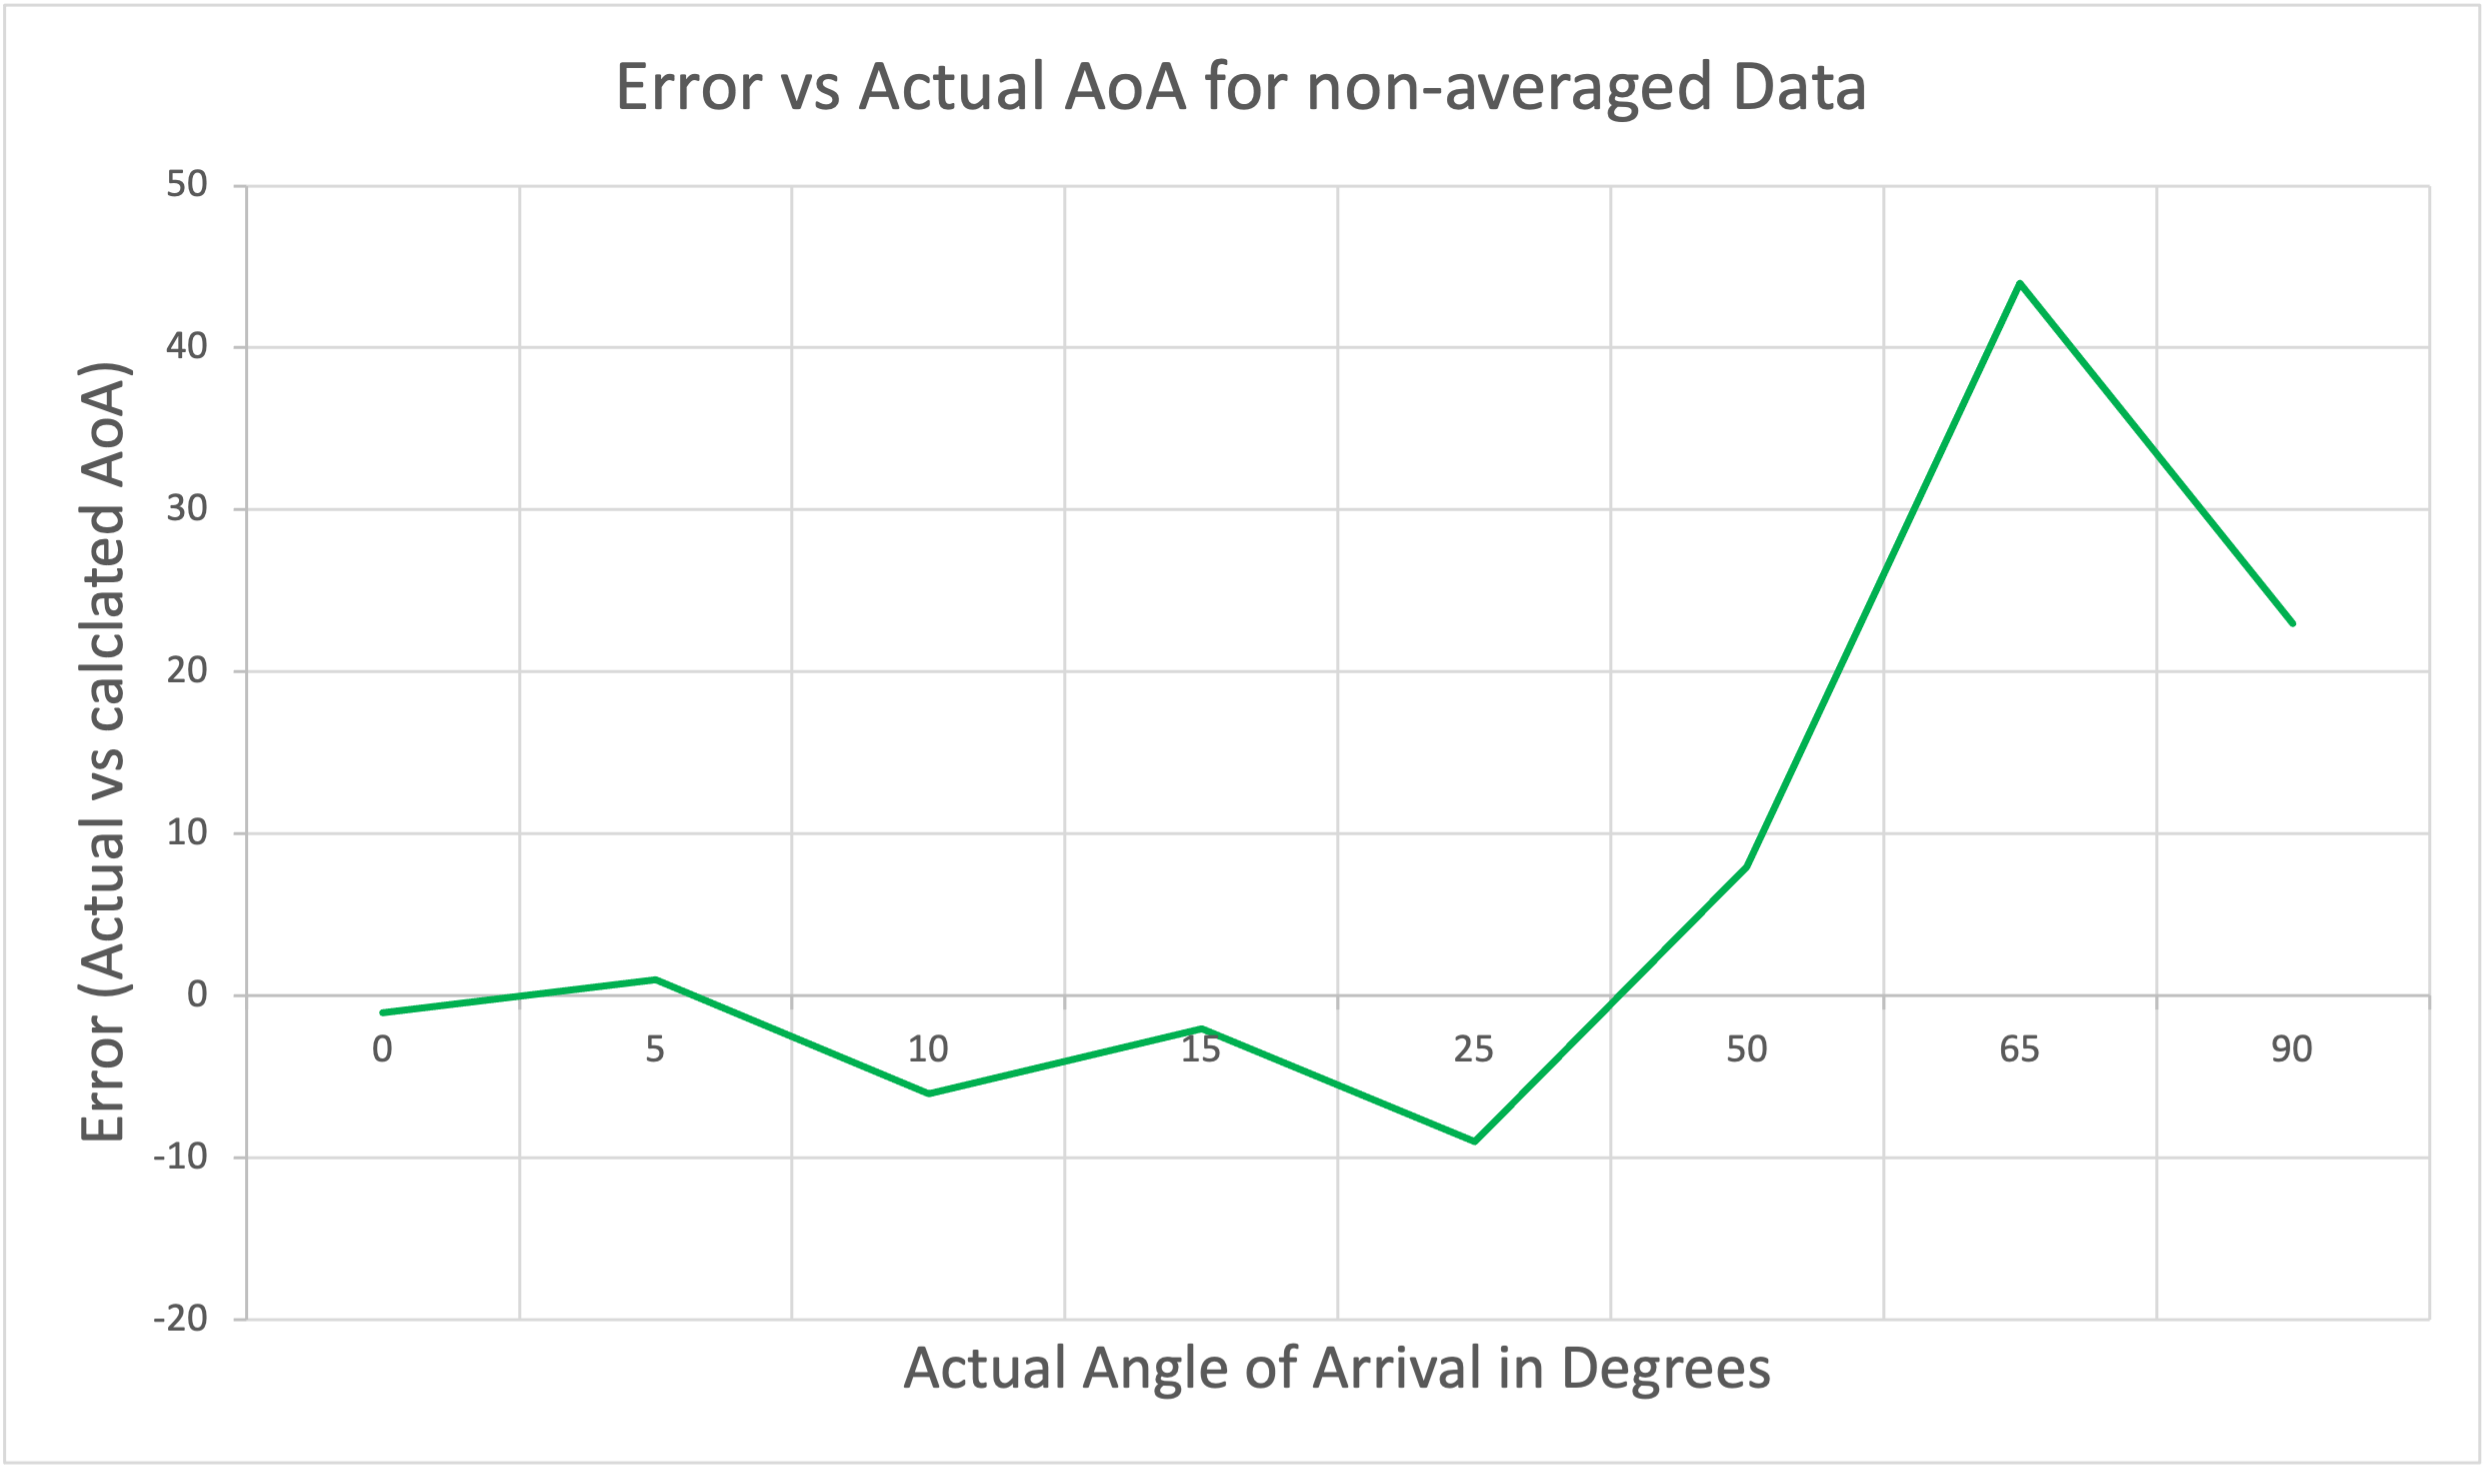
\includegraphics[width=0.92\textwidth]{Images/plots/sensitivity-nonaverage.png} 
\caption{Error sensitivity of prototype without averaging} 
\end{subfigure}\vspace{10pt}

\begin{subfigure}[b]{\linewidth} 
\centering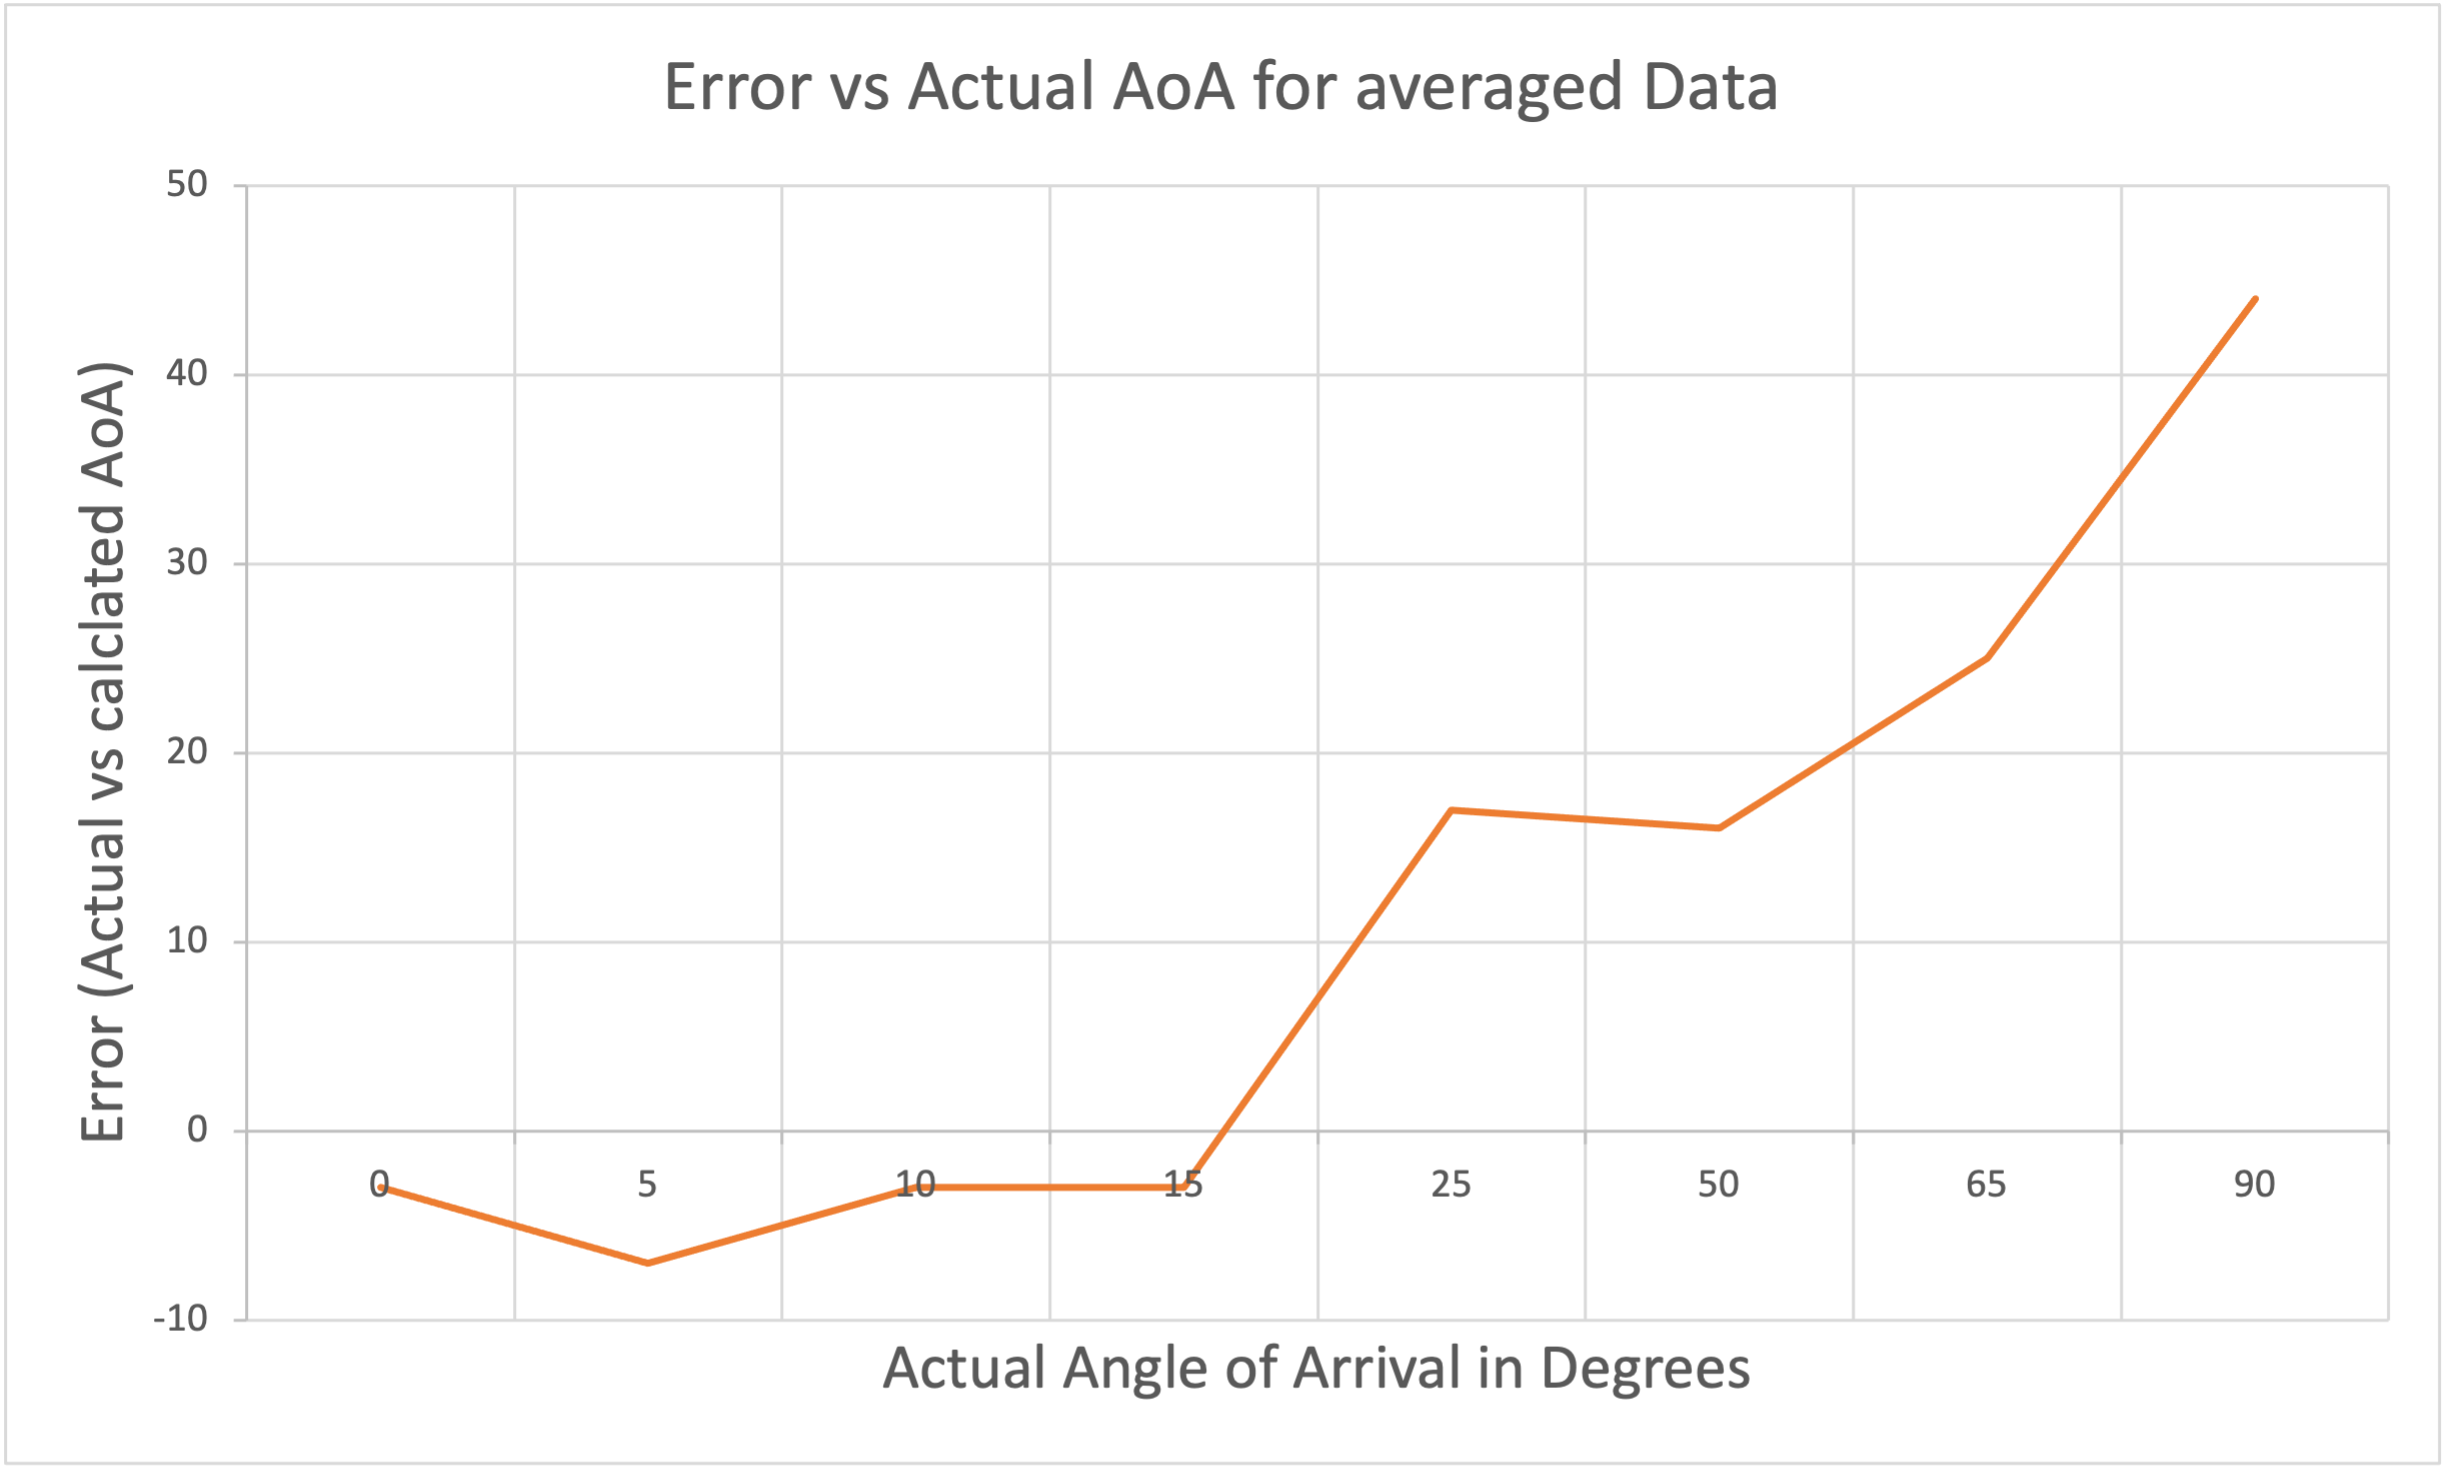
\includegraphics[width=0.45\textwidth]{Images/plots/sensitivity-average.png} 
\caption{Error sensitivity of prototype with averaging} 
\end{subfigure} 
\caption{Error sensitivity of actual AoA vs the calculated \gls{AoA}} 
\end{figure} 

Figure \ref{fig:sim-error}, clearly shows the error between the calculated \gls{AoA} value and the actual \gls{AoA} decreases as the angle increases. This is to be expected as at bigger angles, a small change in the angle induces a greater \gls{pd}. 

However in the system prototype, both with averaged and non-averaged data, not only is the error rate higher, but the error increases in increased angles. For both data sets, the system was accurate until 25 degrees, from which the error increases significantly. A possible reason for this is the quantization of the \gls{sdr} \gls{adc}, which is only 12-bits. The quantization error, as a result, will cause rounding in the \gls{pd}.

The error is less in the averaged data-set, which is expected. However, there are cases where phase extraction without averaging extracts a more accurate \gls{pd} on the first iteration. 
Both the simulation and prototype did not agree with the hypothesis.

%---------------------------------
% Issues 
%---------------------------------
\section{Issues}

While the overall aim to prove that movement of the transmission source would induce a change in phase measured at the \gls{rx} antennas was a success, several issues during the validation process arose. 

Firstly, the GNU Radio \textsc{Python} code abstracted a significant portion of the function calls and scheduling, which for testing was helpful, however this allowed little control over the delays and synchronisation of the received samples. While \ref{fig:time-align} shows a correlation of signals in the time domain at each antenna, this was not always the case. Due to time limitations of this project, further investigation could not be carried out on this. Perhaps luckily, the signals did in fact seem to be aligned, and a phase change was measured, as shown in table \ref{tab:phase-results1}.

Secondly, an unknown phenomenon occurred in the sampled data received from the LimeSDR as shown in figure \ref{fig:lime-clipping}. This always occurred at the same sample position and for the same number of samples in both files (from both \gls{rx} \gls{adc}. This is strange and most certainly needs further investigation, but posturing a guess, it is due to aligned within the \gls{sdr} \gls{fpga} for \gls{mimo}.

\begin{figure}[h]
    \centering
    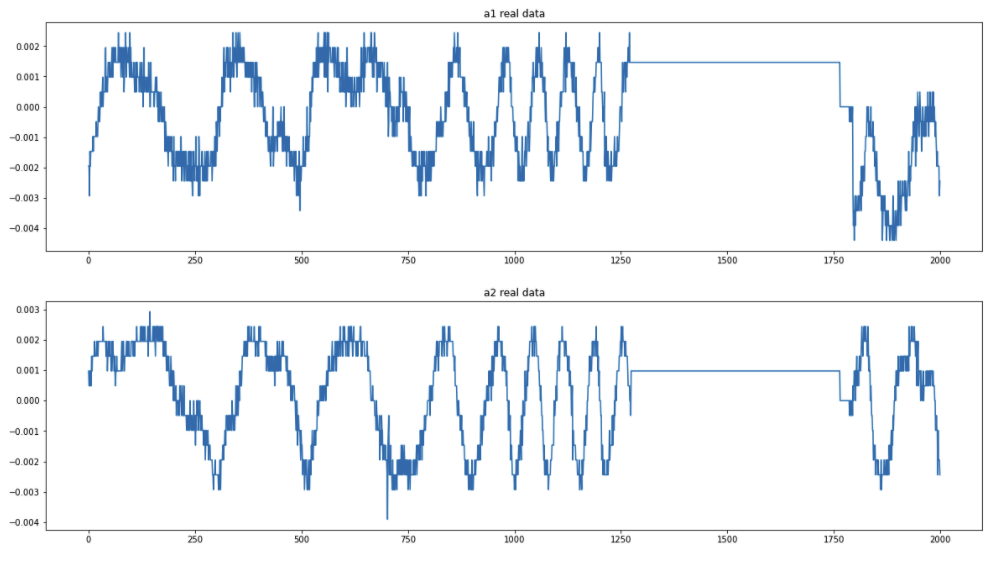
\includegraphics[width=0.9\textwidth]{Images/plots/weirdclipping.png}
    \caption{An issue with pausing of sampled data within the LimeSD}
    \label{fig:lime-clipping}
\end{figure}

Thirdly, overheating of the LimeSDR prevented sample capturing at 20MHz for periods longer than 10 to 15 seconds. If left running, the board temperature would increase, and data would stop streaming to the host computer. This hampered testing, however, the board is capable of transmission rates at the speed if the code is further optimised and bloated GNU Radio replaced with C++ \gls{API}.

Finally, while the Raspberry Pi 4 is capable and well suited to this project, additional heat-sinks and perhaps a cooling fan should be added as the CPU temperature hindered performance. For real-time graphing, this significantly slowed down testing. 


%---------------------------------
% Summary
%---------------------------------
\section{Summary}
This chapter presented a series of validation tests falling into four broad categories, all designed to test and validate the \gls{df} system, with a specific focus on a change in the measured phase. Firstly, a simulated environment and \gls{pd} was validated for the workings of algorithms and calculations. Secondly, the proof of sampled, time-aligned signals was validated for the system prototype, and phase results were subsequently collected. Thirdly, a rudimentary statistical analysis of the collected results was discussed. Finally, the sensitivity of phase measurement to the incident angle is measured. In all validation tests, tables, plots and graphs are provided for explanation where necessary. 

The results for the tests convincingly prove that the prototype system is capable of measuring a change in phase, producing a \gls{pd} between two \gls{rx} signals, and this is capable of \gls{df}. 

% ----------------------------------------------------
\ifstandalone
\bibliography{Bibliography/References}
\printnoidxglossary[type=\acronymtype,nonumberlist]
\fi
\end{document}
% ----------------------------------------------------